%\documentclass{article}
%\usepackage[utf8]{inputenc}

\documentclass[12pt]{article}
\usepackage{graphicx} % This lets you include figures
\usepackage{hyperref} % This lets you make links to web locations
\graphicspath{ {./images/} }

\usepackage[rightcaption]{sidecap}
\usepackage{caption}
\usepackage{subcaption}
\usepackage{hyperref}

\usepackage{float}

\usepackage{imakeidx}

\makeindex


\title{AnaEE Interface Manual}
\author{Beau De Clercq}
\date{July 2019}

\begin{document}
\maketitle{}

\tableofcontents

\clearpage
\newpage

\section{Setting Up for the first time}
\subsection{Prerequisites}
In order to be able to run the interface locally, a Python distribution of version 3.6 or higher needs to be installed and has to be on the system PATH.\\
Python can be found at \url{https://www.python.org/downloads/}. By downloading the installer and selecting the "Add to Path" option when executing it the prerequisite will be fulfilled.
\subsection{On Windows}
Installation can be done in 2 ways.
\begin{itemize}
	\item Automatically by running the provided executable.
	\item Manually by installing Visual Studio found at \url{https://visualstudio.microsoft.com/downloads/} and restarting the computer. 
\end{itemize}
\subsection{On Mac}
Ensure that the \texttt{gcc} command works. If this is not the case, follow the instructions provided by Apple to resolve this problem. Afterwards the user can execute the provided bash script in a terminal.
\subsection{On Linux}
Execute the provided bash script in a terminal.
\newpage
\section{Starting the interface}
\subsection{On Windows}
Execute the provided bat script in a terminal.
\subsection{On Mac or Linux}
Execute the provided bash script in a terminal.
\newpage

\section{Usage}
\subsection{Adding a record}
\begin{center}
	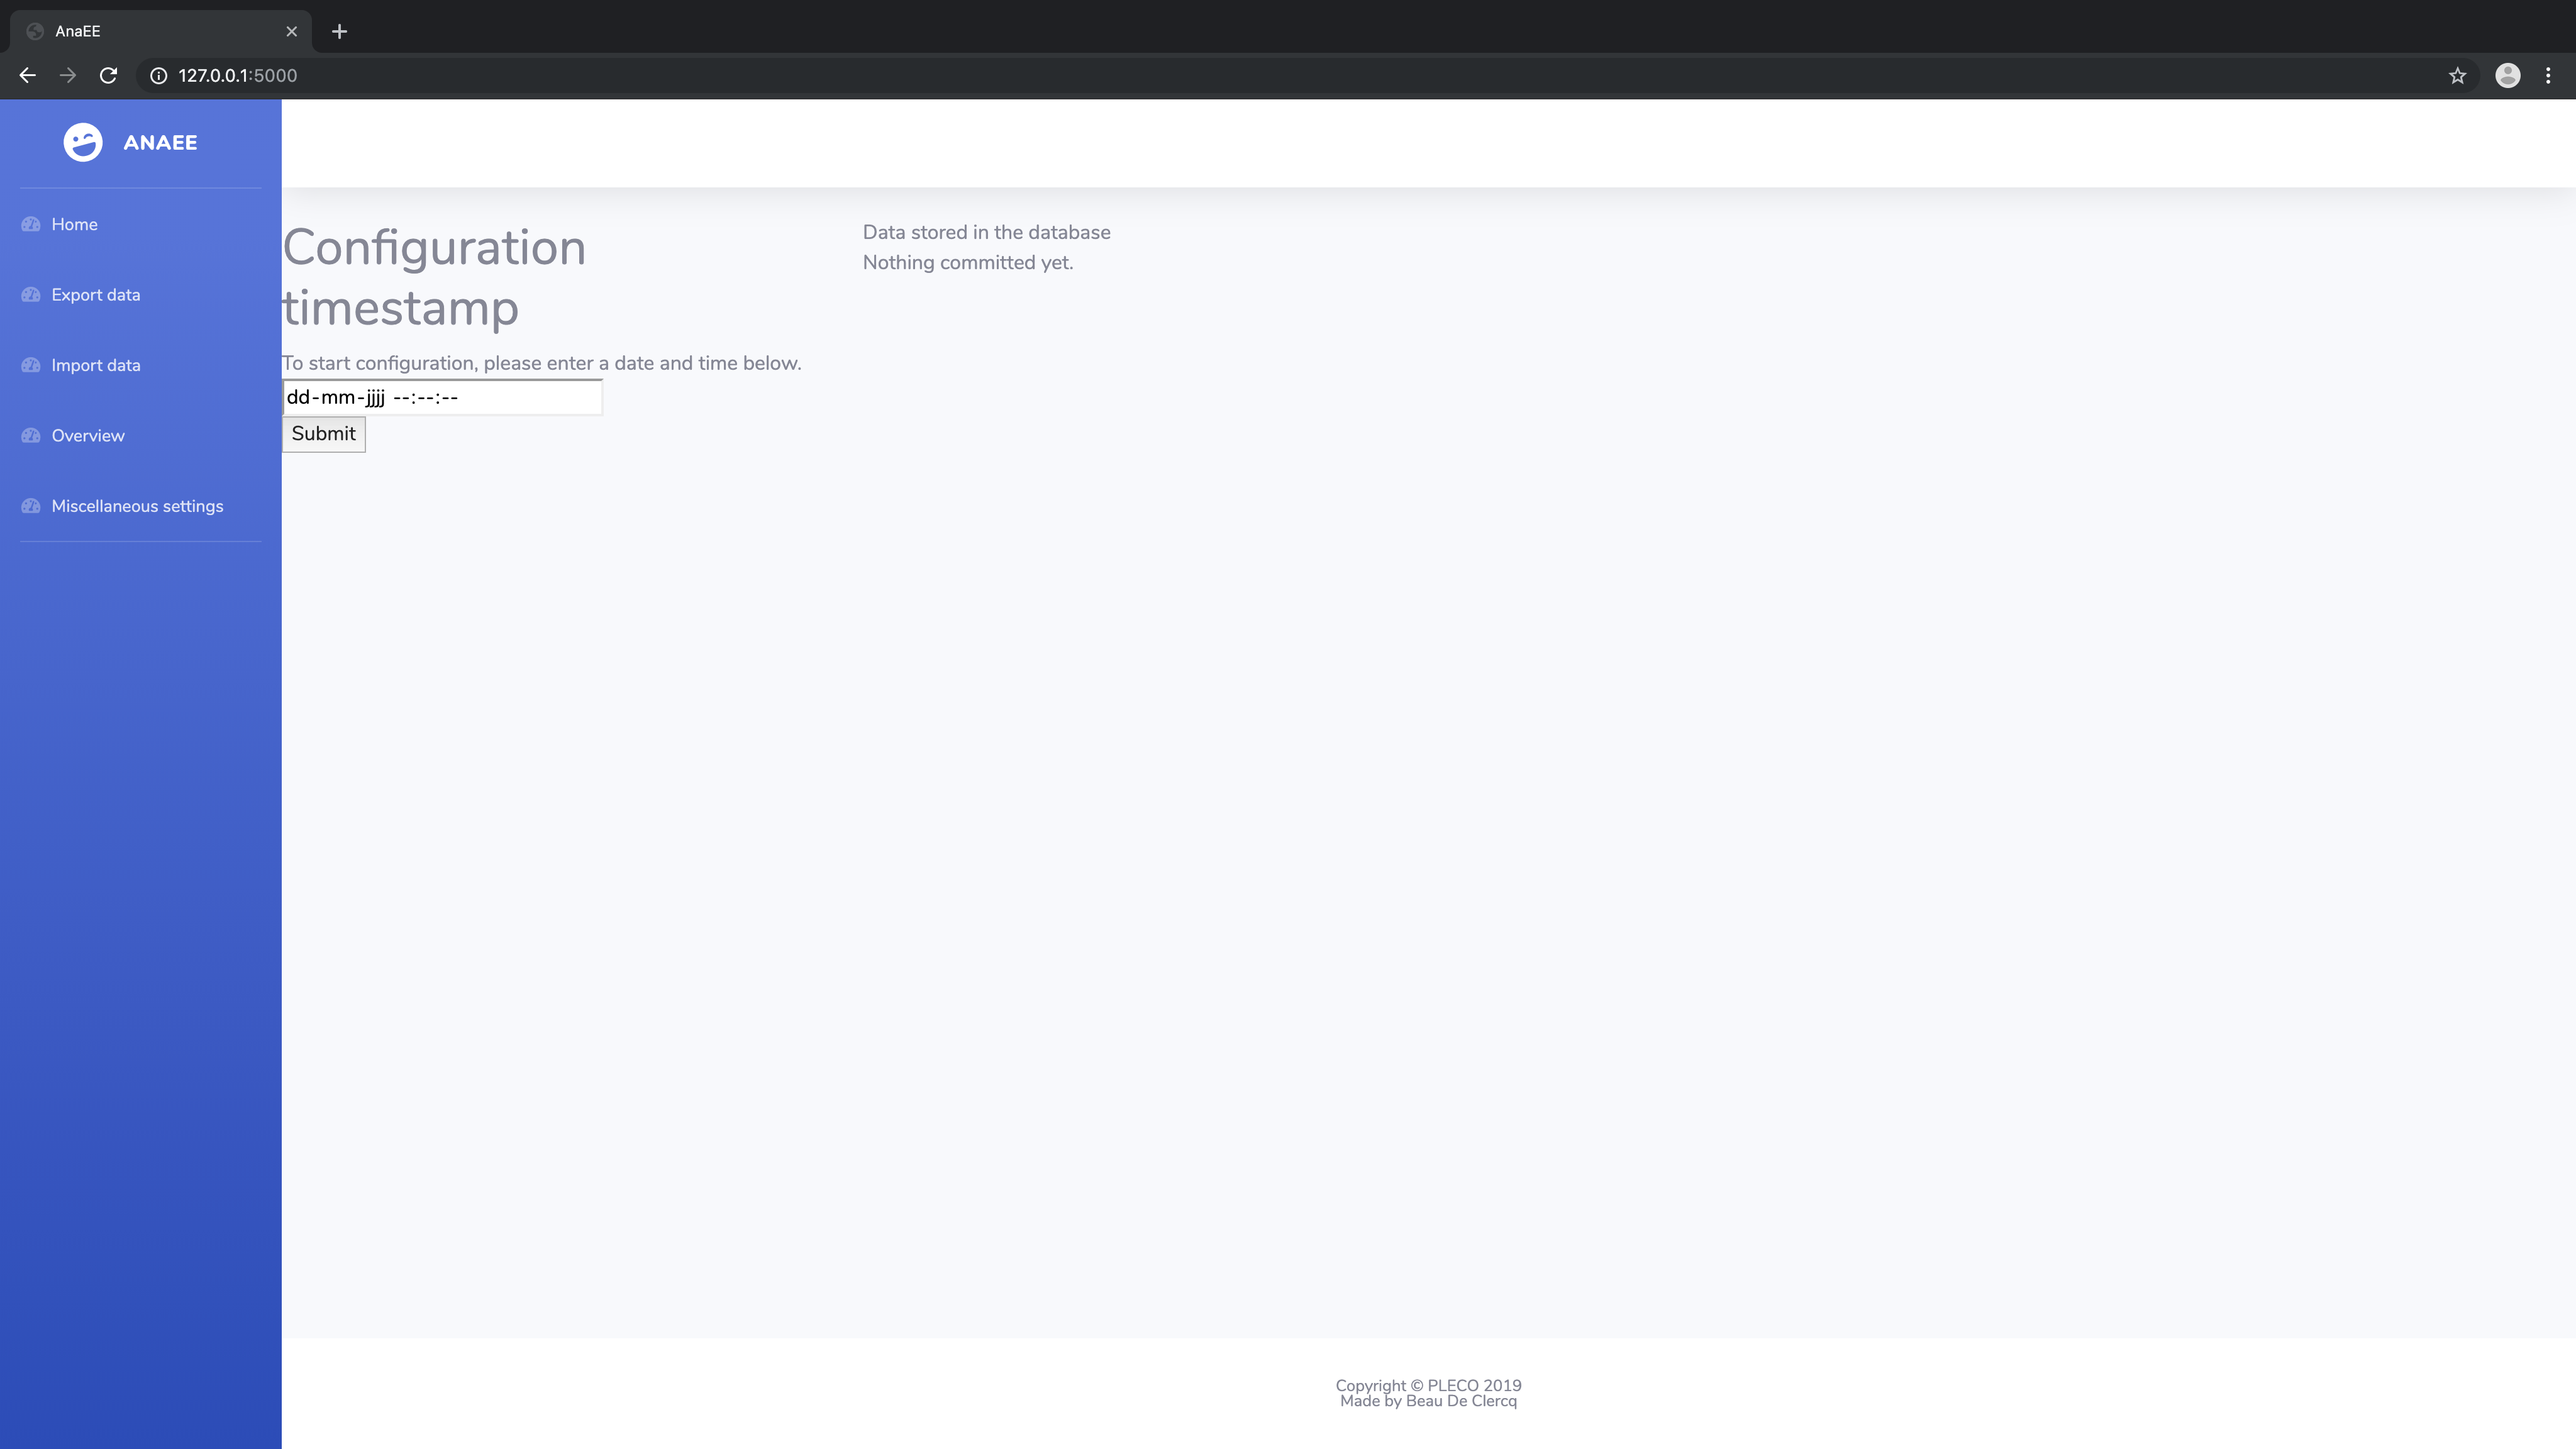
\includegraphics[width=\linewidth]{images/Home_screen_no_data.png}
	\captionof{figure}{Home screen}
\end{center}
A new configuration can be added to the database by filling in a configuration timestamp and clicking the \lq Submit\rq button on the home screen. This will take the user to the configuration screen.\\
\begin{center}
	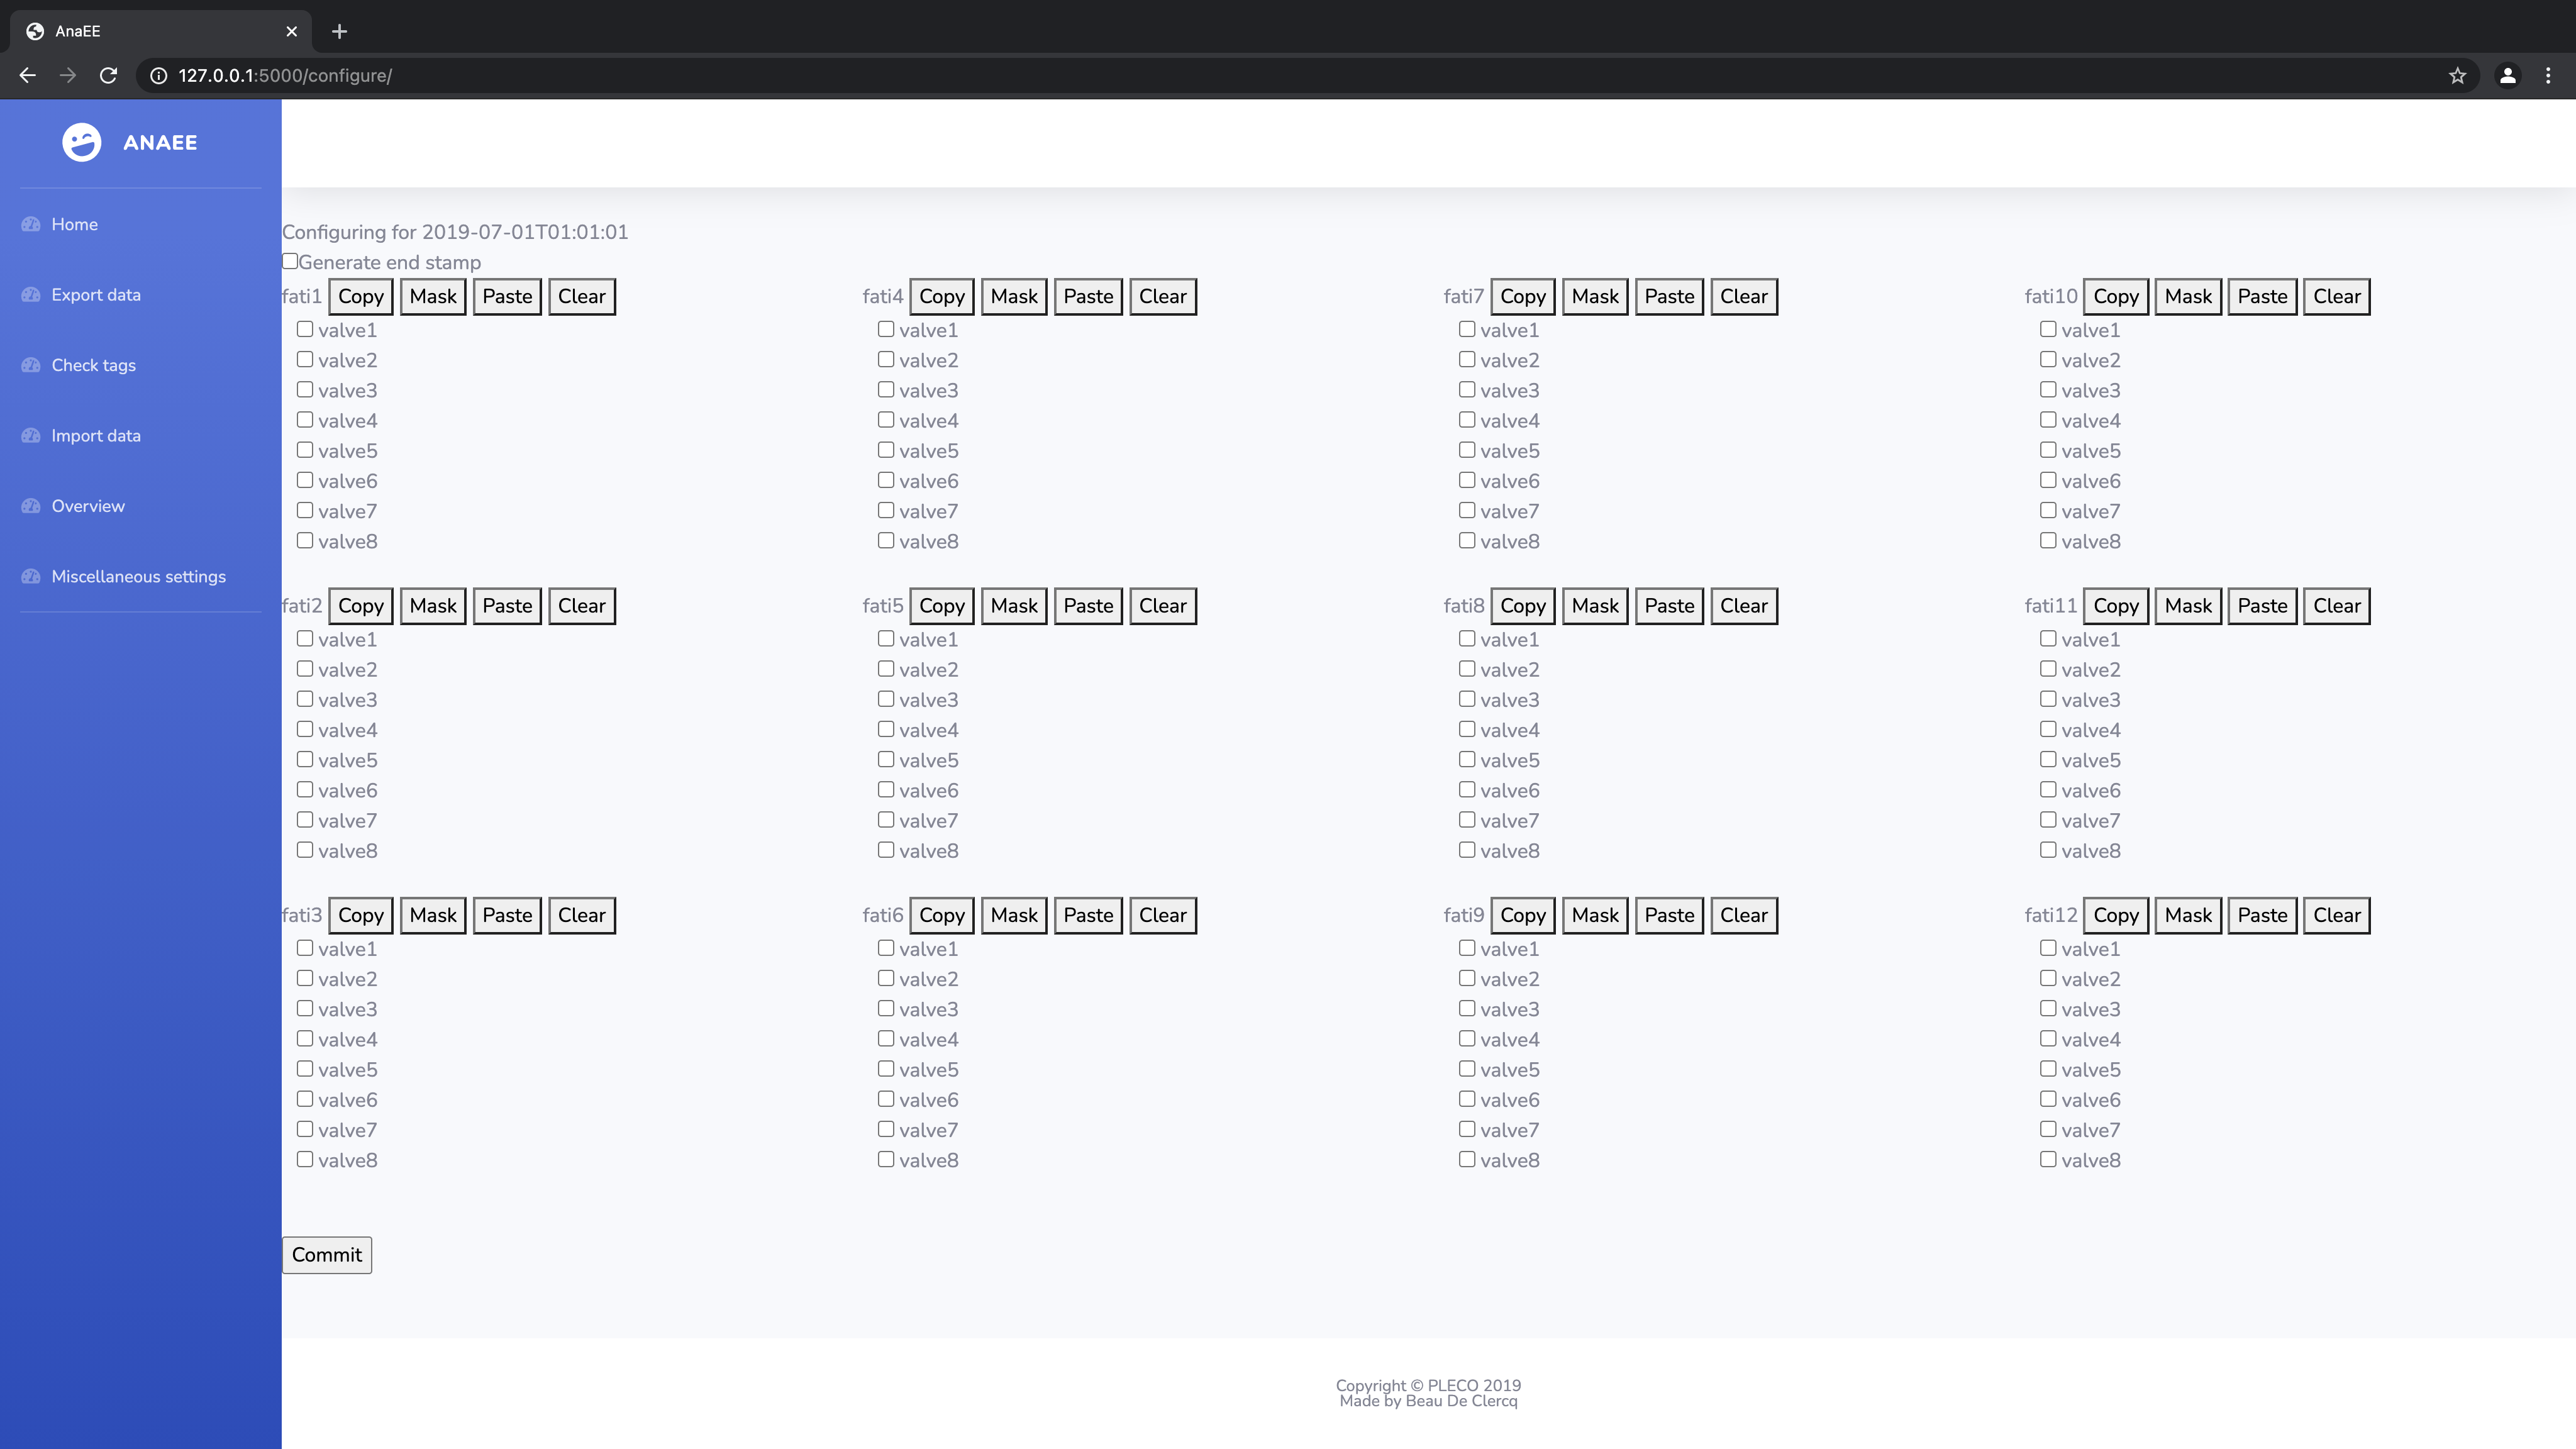
\includegraphics[width=\linewidth]{images/Empty_config_screen.png}
	\captionof{figure}{Configuration screen}
\end{center}
In the configuration screen a user can select which valves need to be active at the previously entered date and time.\\
To make this step easier a few options are available.
\begin{itemize}
	\item Copy: copy the configuration of the concerning fati.
	\item Paste: paste a previously copied configuration to the concerning fati.
	\item Mask: a special sort of Paste, this button will add the copied check-boxes to the concerning fati.
	\item Clear: remove all checked boxes from the concerning fati.
\end{itemize}
At the top of the screen the user can select wheter an end-stamp needs to be generated or not. If checked, this end-stamp will be generated based on the specified value in the \lq Miscellaneous settings\rq.\\
If everything is filled in as desired, the configuration can be committed to the database by clicking the \lq Commit\rq button. Afterwards the user will be taken back to the homepage.

\subsection{Editing a record}
\begin{center}
	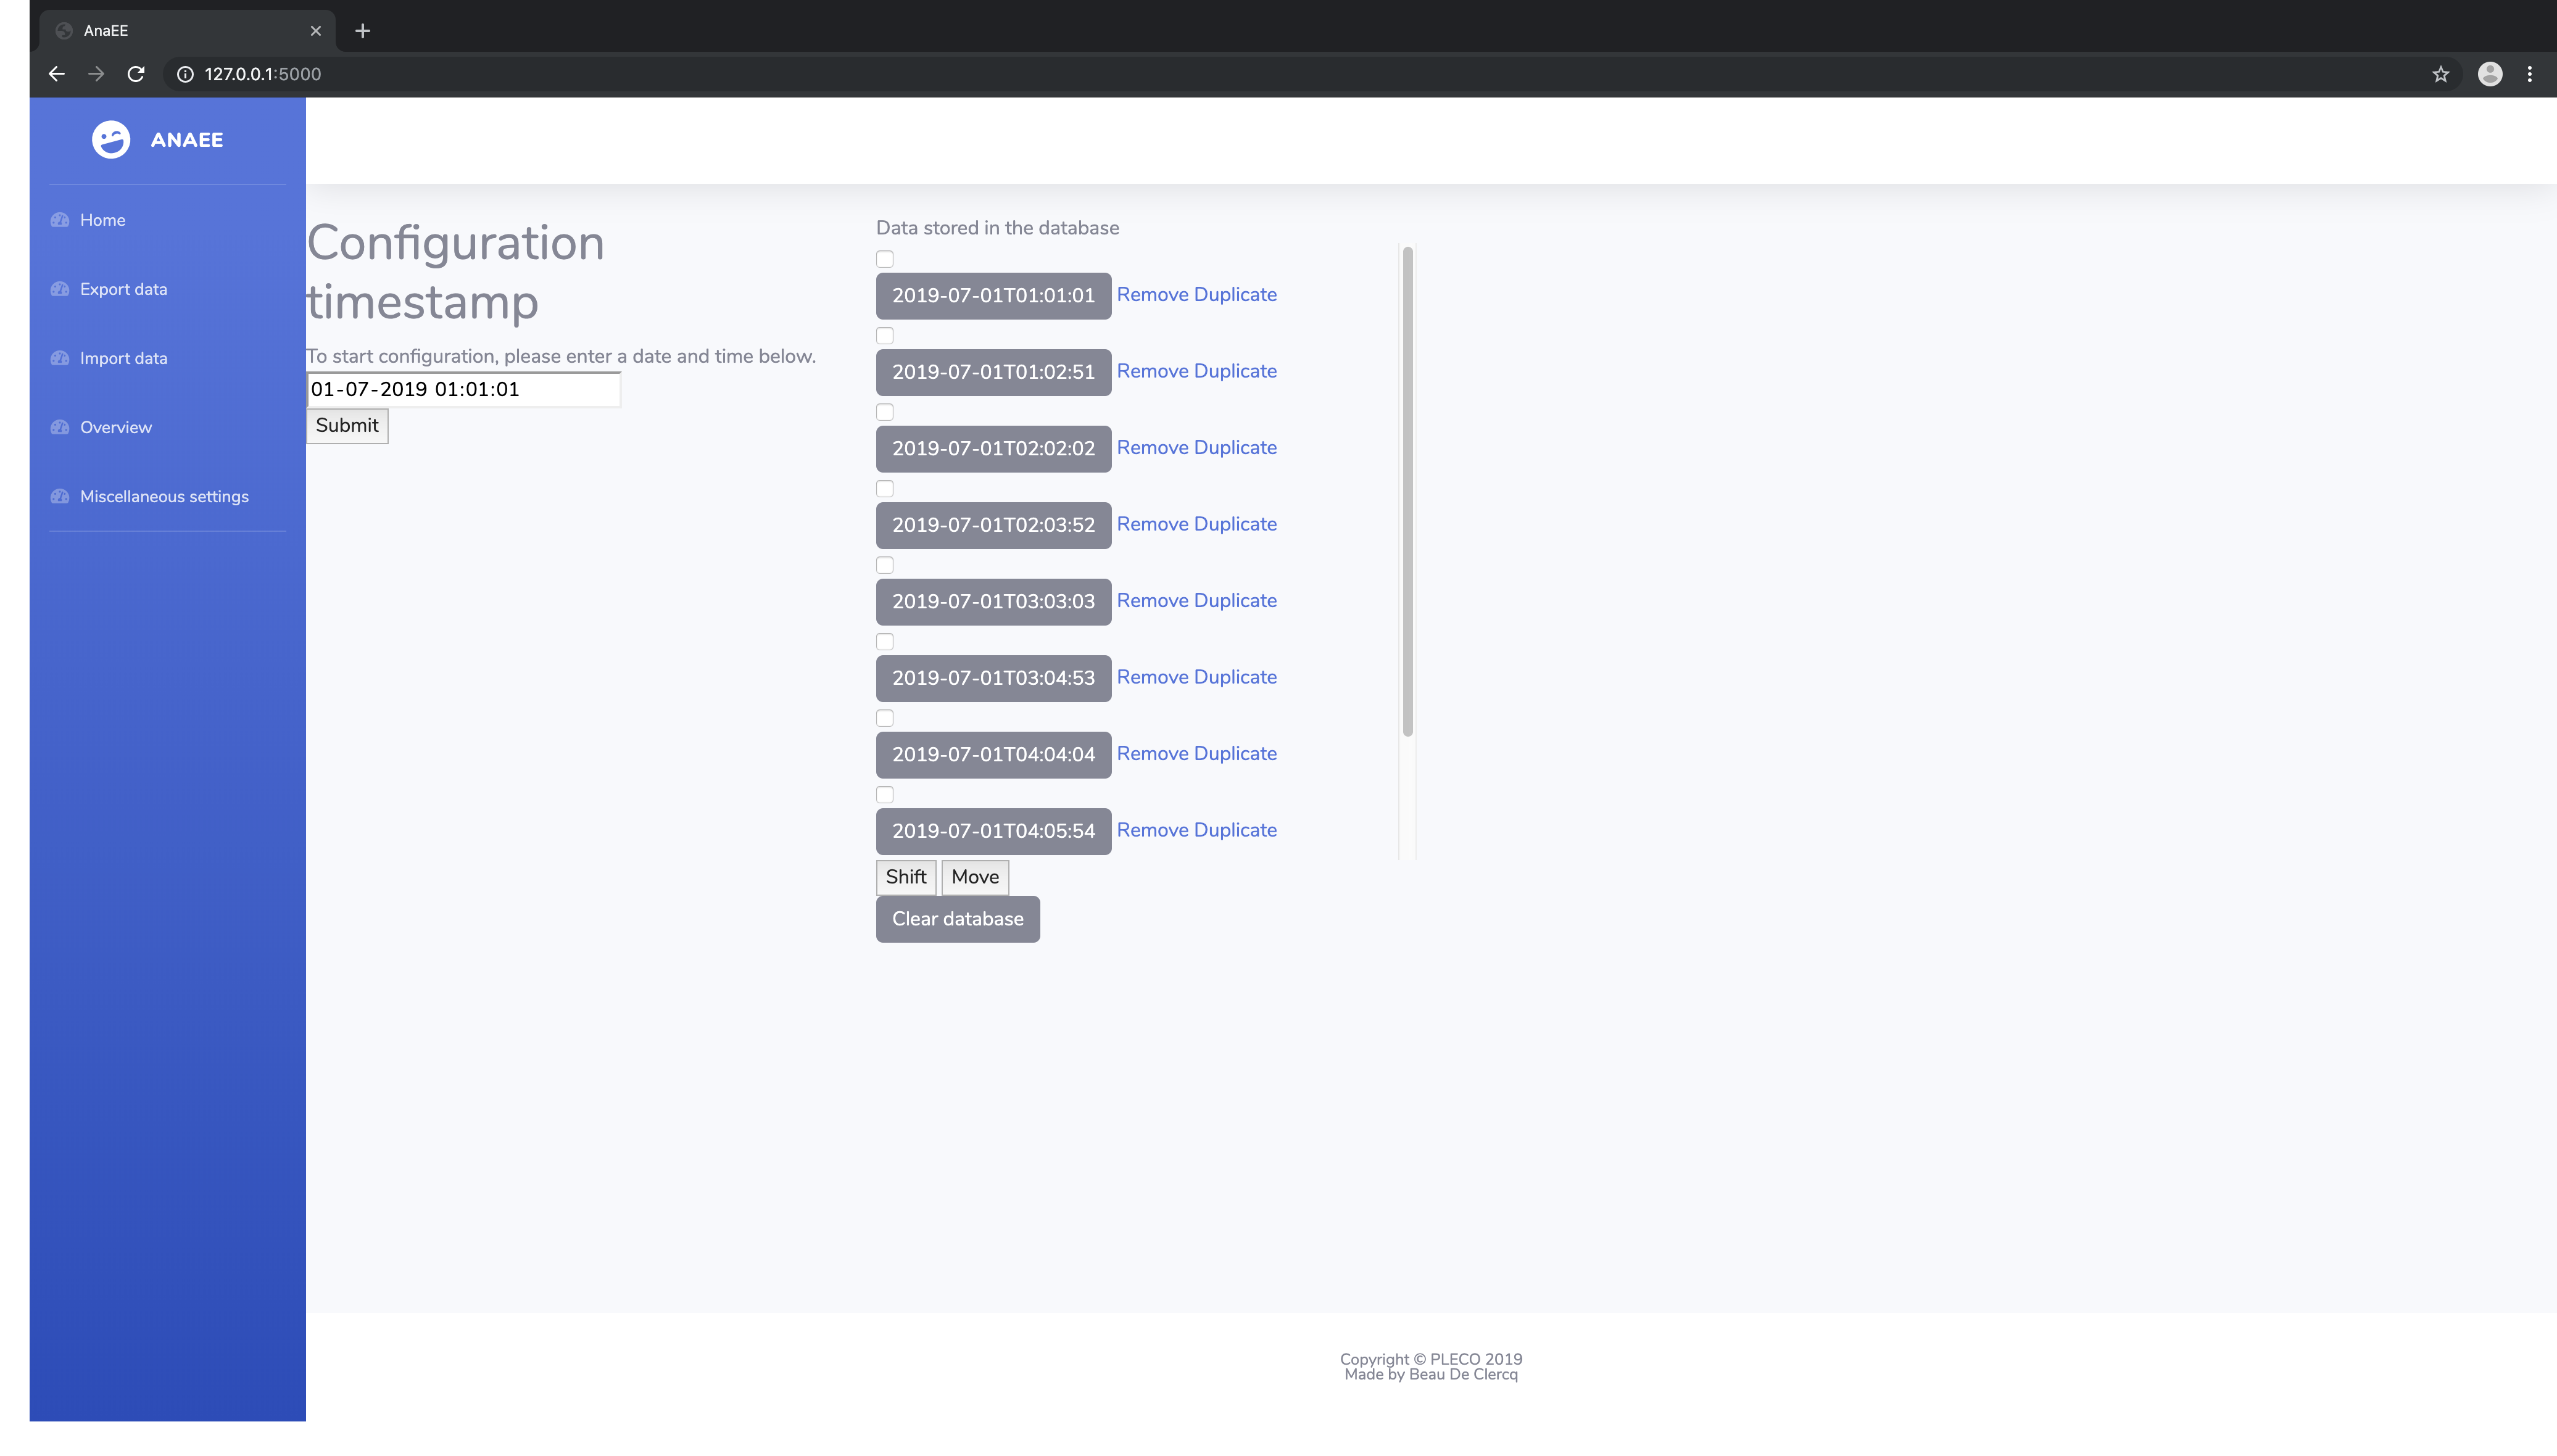
\includegraphics[width=\linewidth]{images/Edit_options.png}
	\captionof{figure}{Ways to edit a record}
\end{center}
There are 2 ways to edit a existing configuration.
\begin{itemize}
	\item Clicking on the record when at the homepage.
	\item Insert the date and time as configuration timestamp at the homepage.
\end{itemize}
Both options will open the configuration screen with the previous data loaded and ready for editing.\\
To preserve the changes made, the record has to be committed again.

\subsection{Removing a record}
\begin{center}
	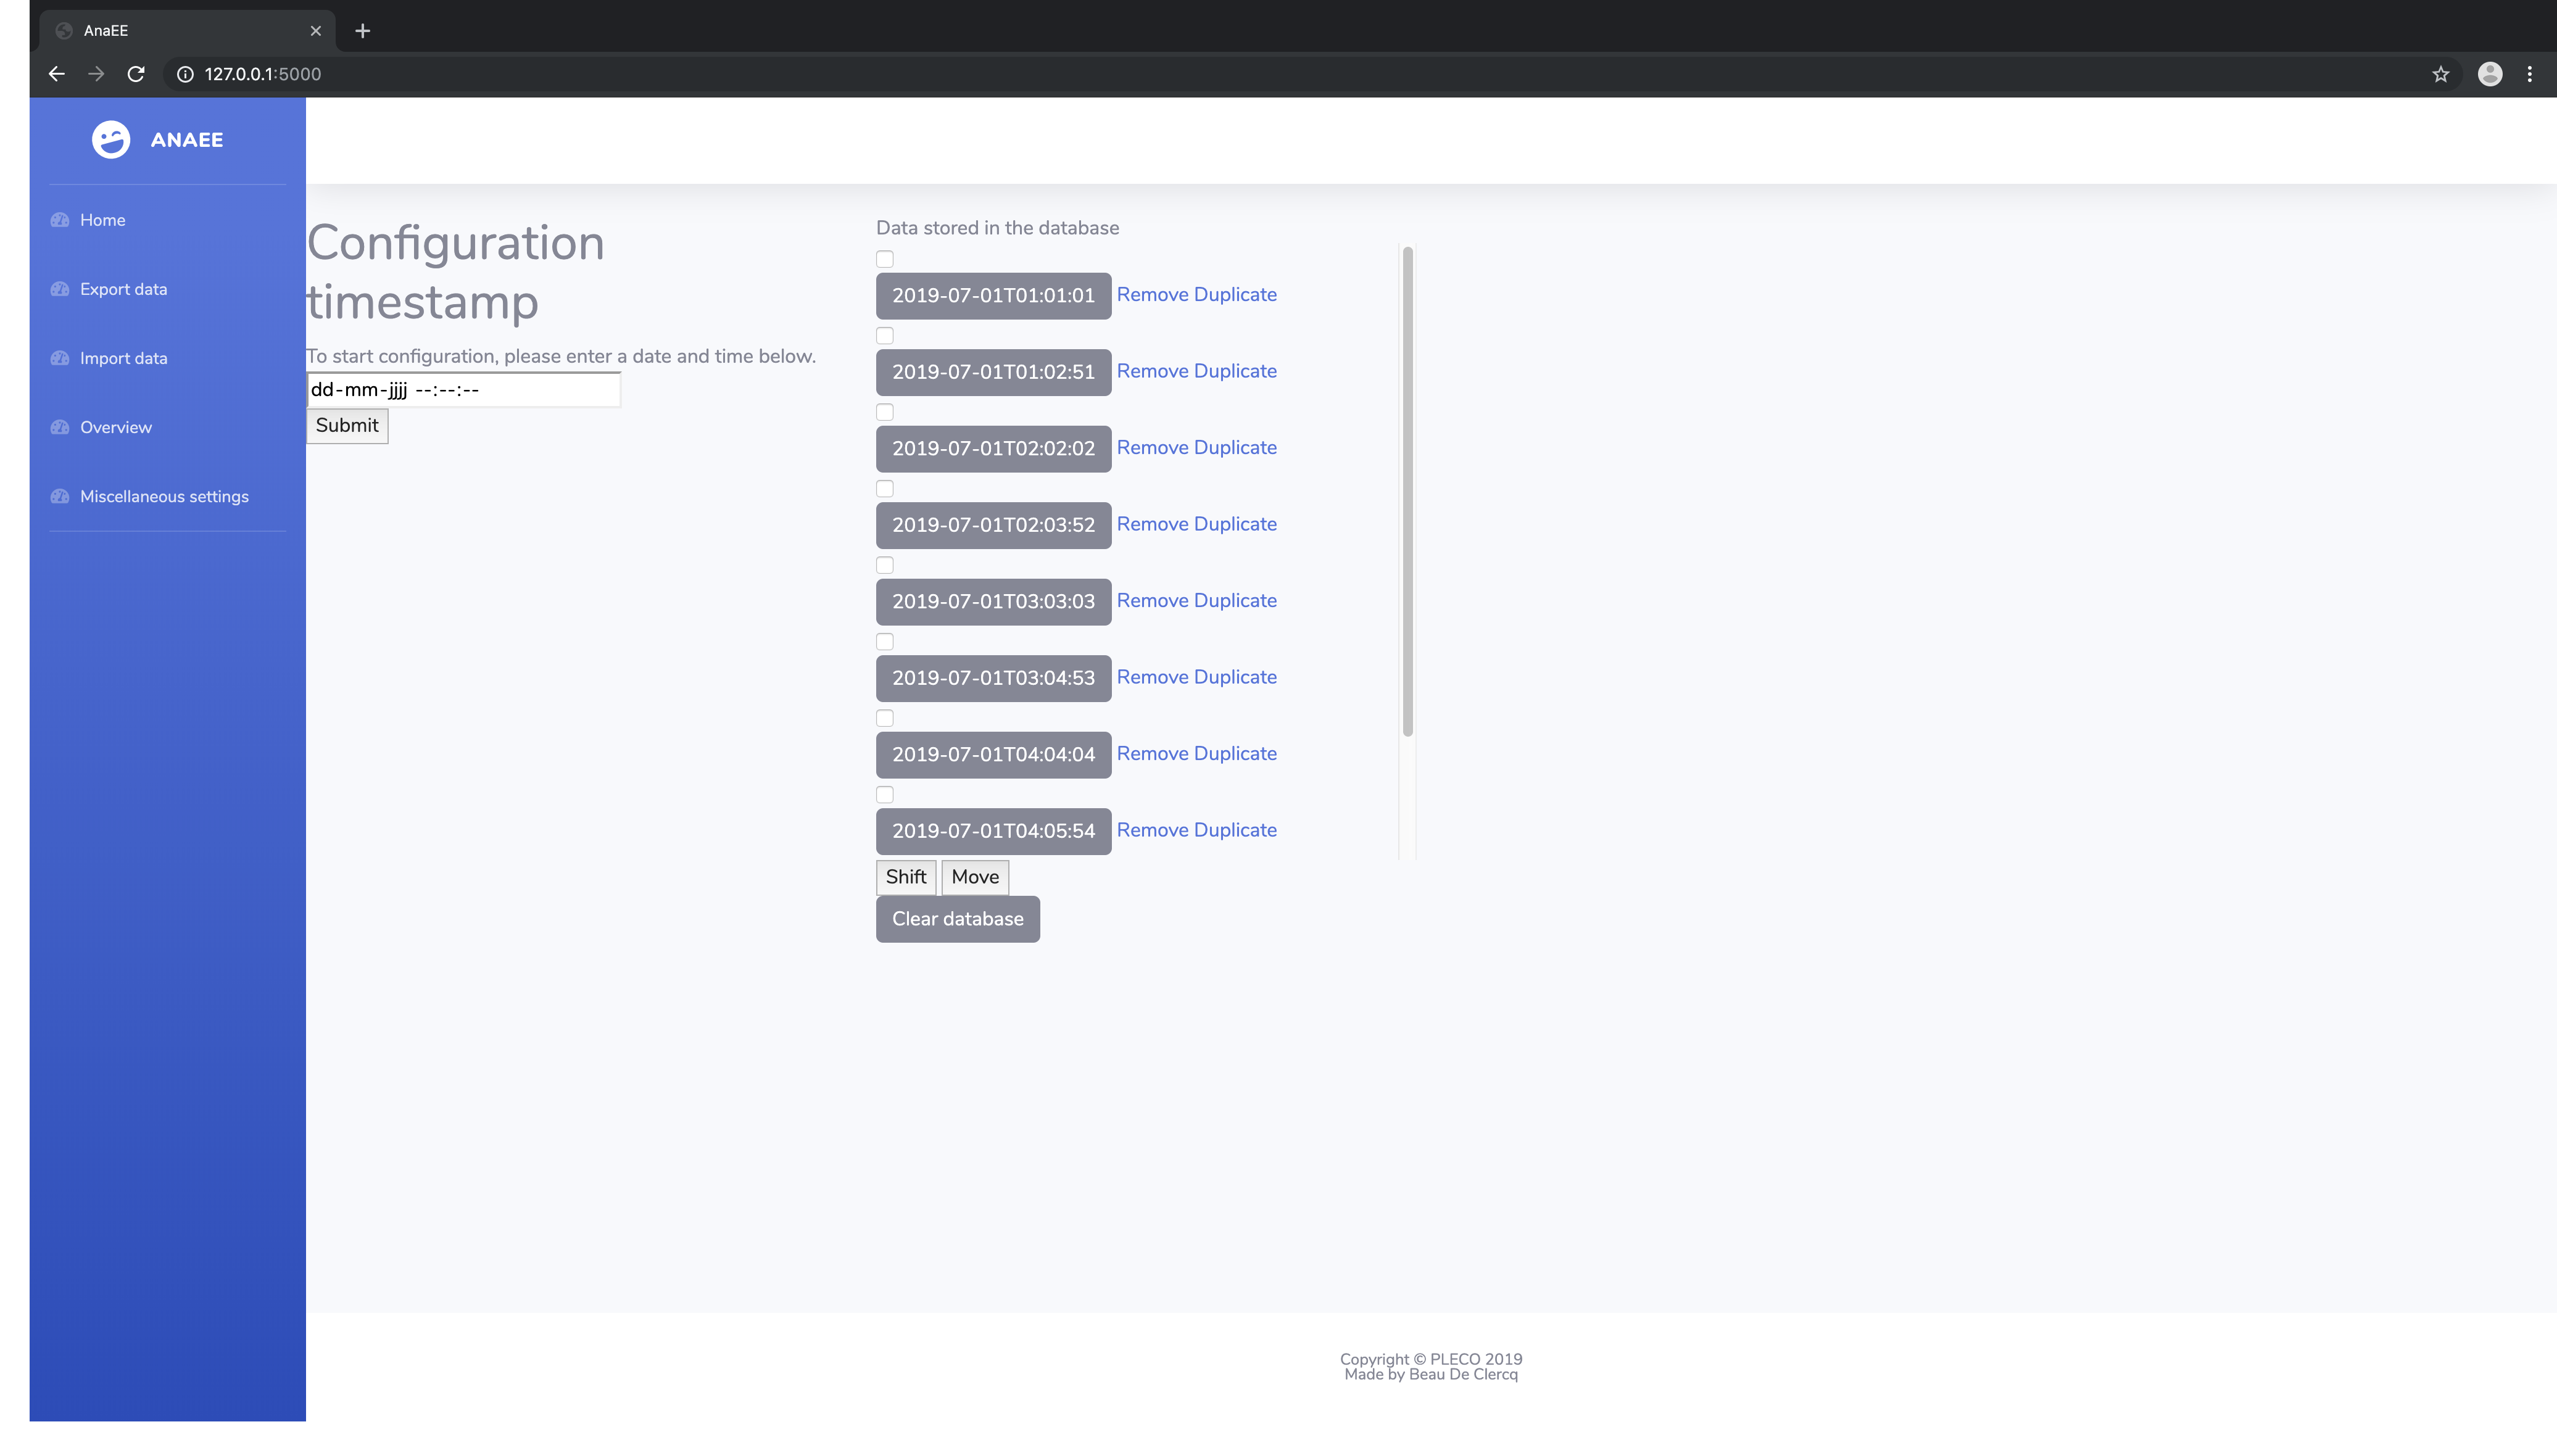
\includegraphics[width=\linewidth]{images/Removing_records.png}
	\captionof{figure}{Ways to remove a record}
\end{center}
A record can be removed in 2 ways.
\begin{itemize}
	\item An individual record can be removed by clicking the \lq Remove\rq button next to the record.
	\item If all records need to be removed at the same time the user can use the \lq Clear database\rq button found beneath the overiew of all records.
\end{itemize}

\subsection{Duplicating record}
\begin{center}
	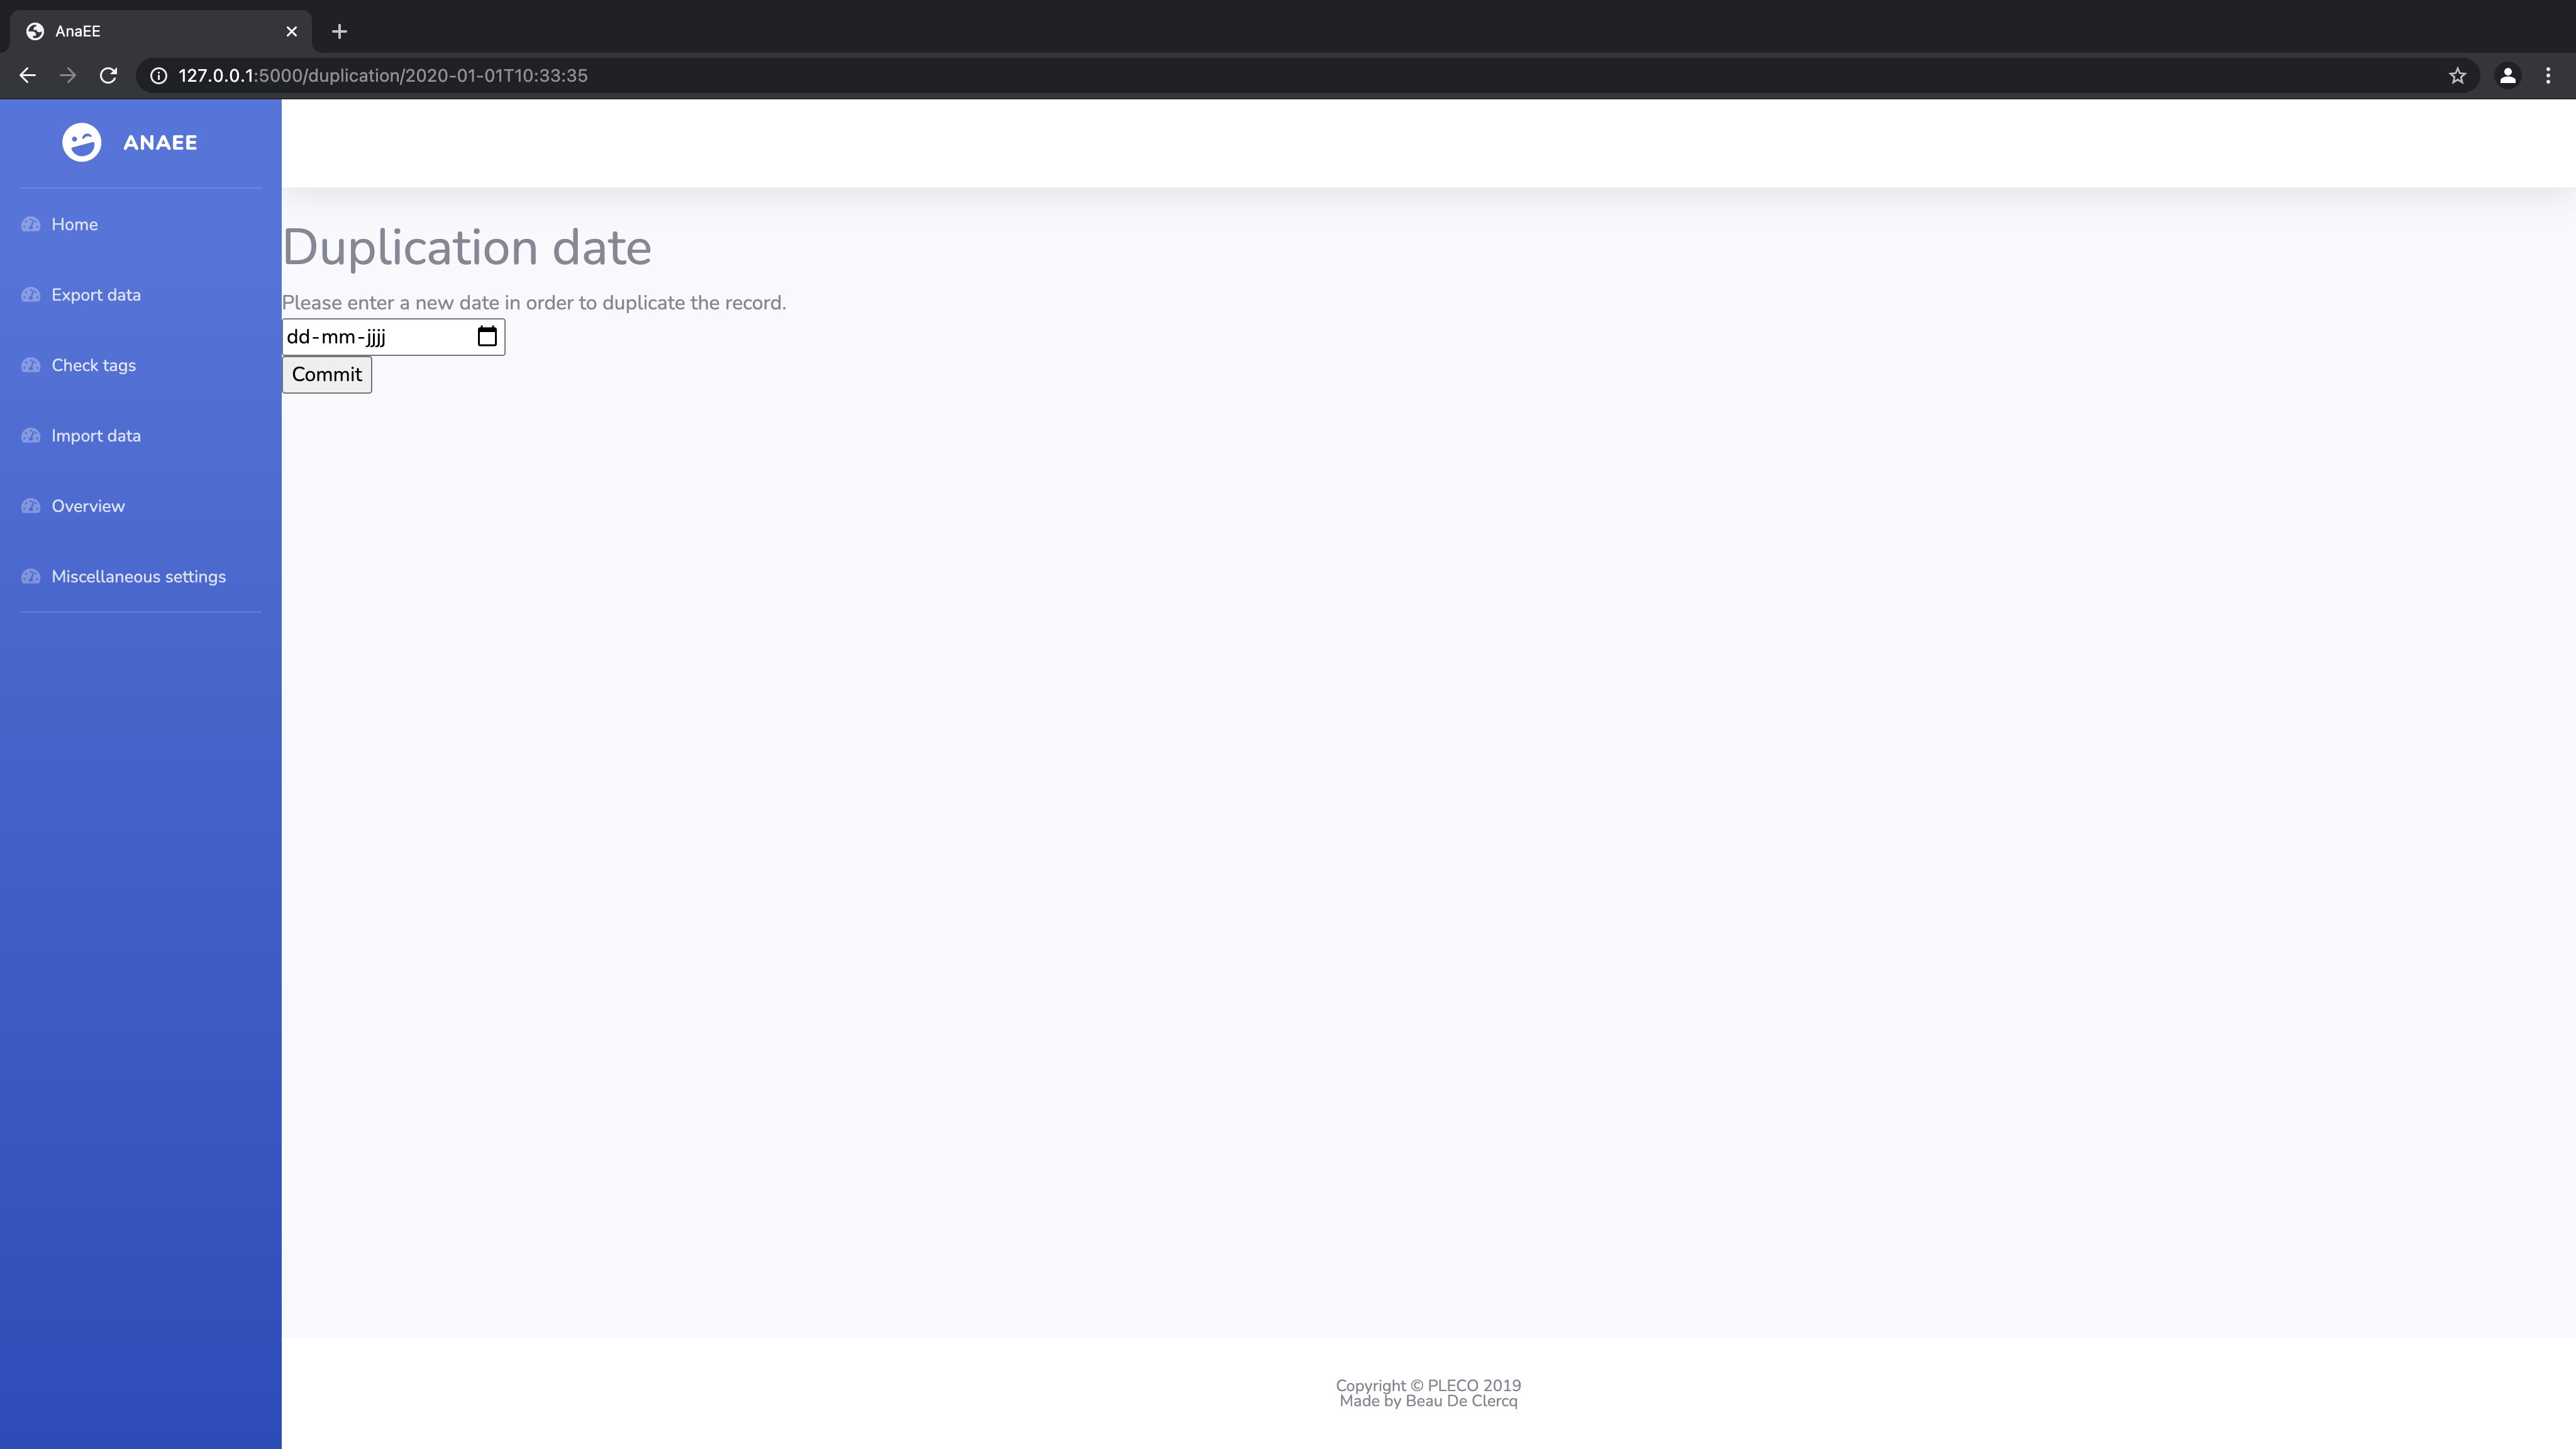
\includegraphics[width=\linewidth]{images/Duplicate_records.png}
	\captionof{figure}{Duplicating a record}
\end{center}
A record can be duplicated by clicking the \lq Duplicate\rq button next to the record.\\
The user will then be taken to a screen where he will be asked to enter a new date. A new record will be inserted containing the new date, the same time as the old record and the same configuration as the old record.

\subsection{Shifting record}
\begin{center}
	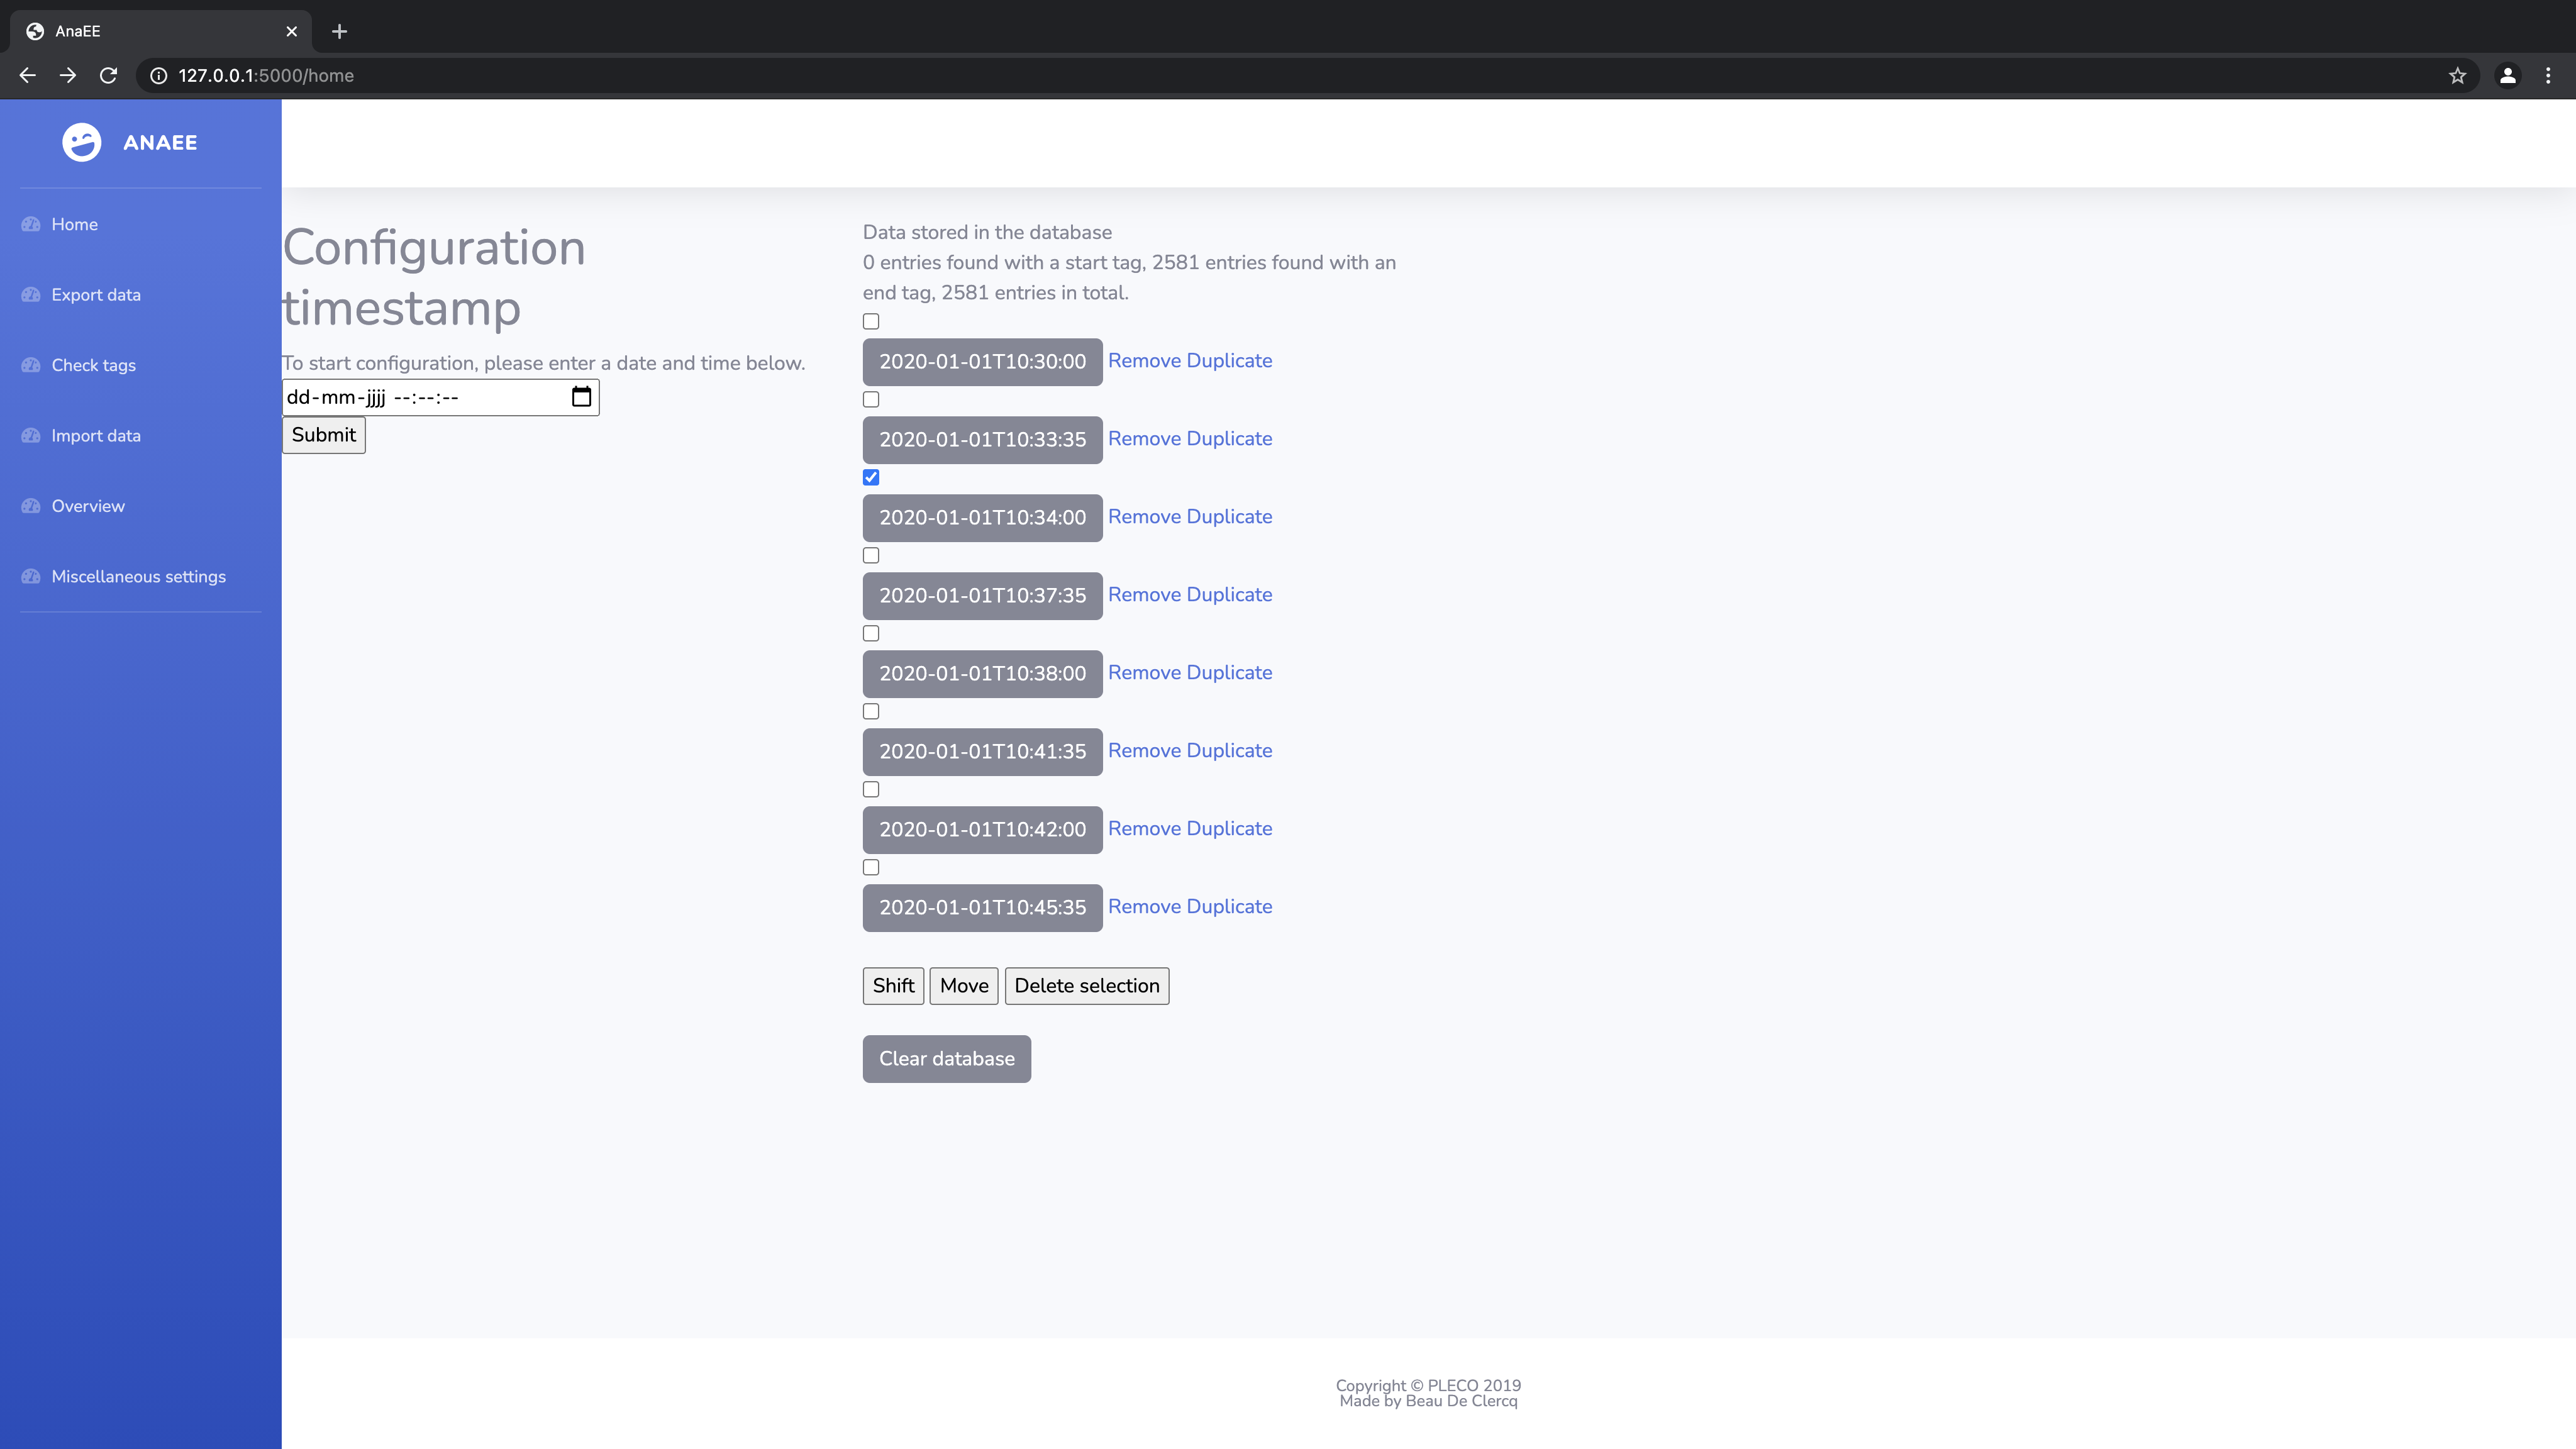
\includegraphics[width=\linewidth]{images/Shift_entries.png}
	\captionof{figure}{Shfiting records}
\end{center}
A series of records can be shifted on the homepage as follows.
\begin{itemize}
	\item Select the first record you want to be shifted.
	\item Make sure no other records are selected.
	\item Click \lq Shift\rq
\end{itemize}
By following this procedure, all records following the selected record will be shifted by the amount of day specified in the \lq Miscellaneous settings\rq tab.

\subsection{Moving records}
\begin{center}
	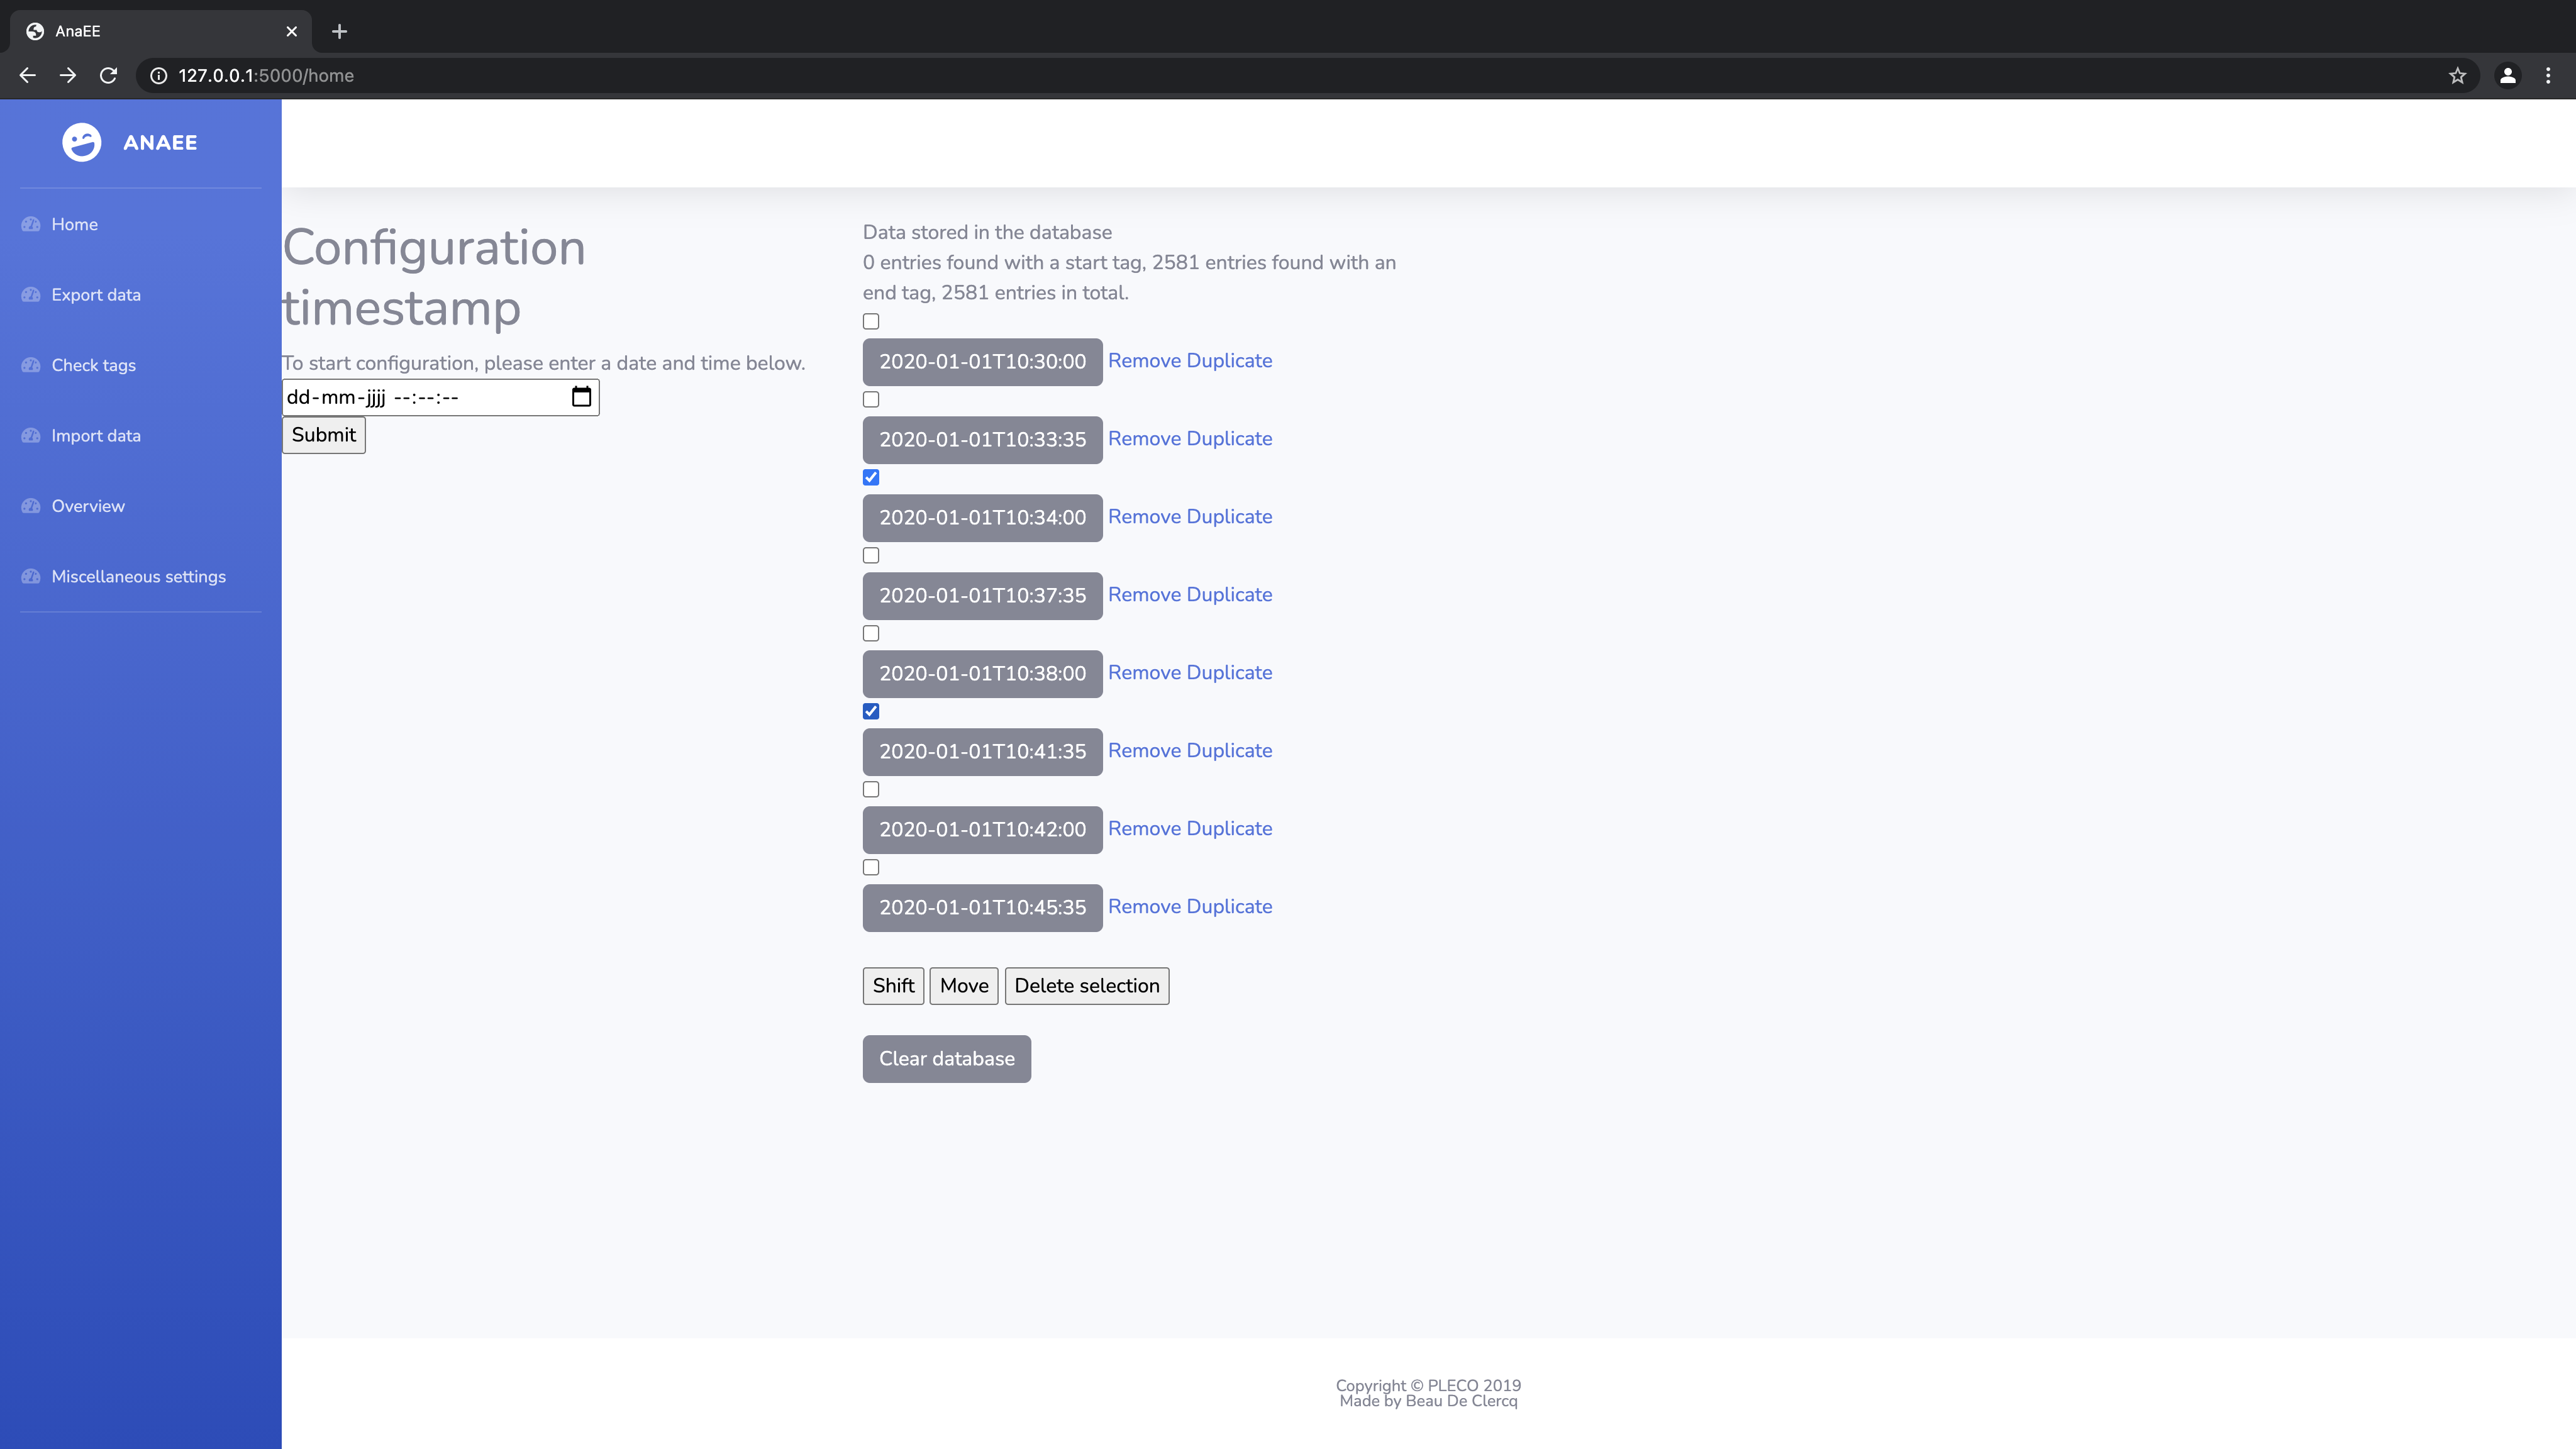
\includegraphics[width=\linewidth]{images/Move_entries.png}
	\captionof{figure}{Moving records}
\end{center}
A series of records can be moved on the homepage as follows.
\begin{itemize}
	\item Select the first  and last record of the series you want to be moved.
	\item Click \lq Move\rq
\end{itemize}
By following this procedure, all records between the selected records will be duplicated by the amount of day specified in the \lq Miscellaneous settings\rq tab.

\subsection{Visual validation}
\begin{center}
	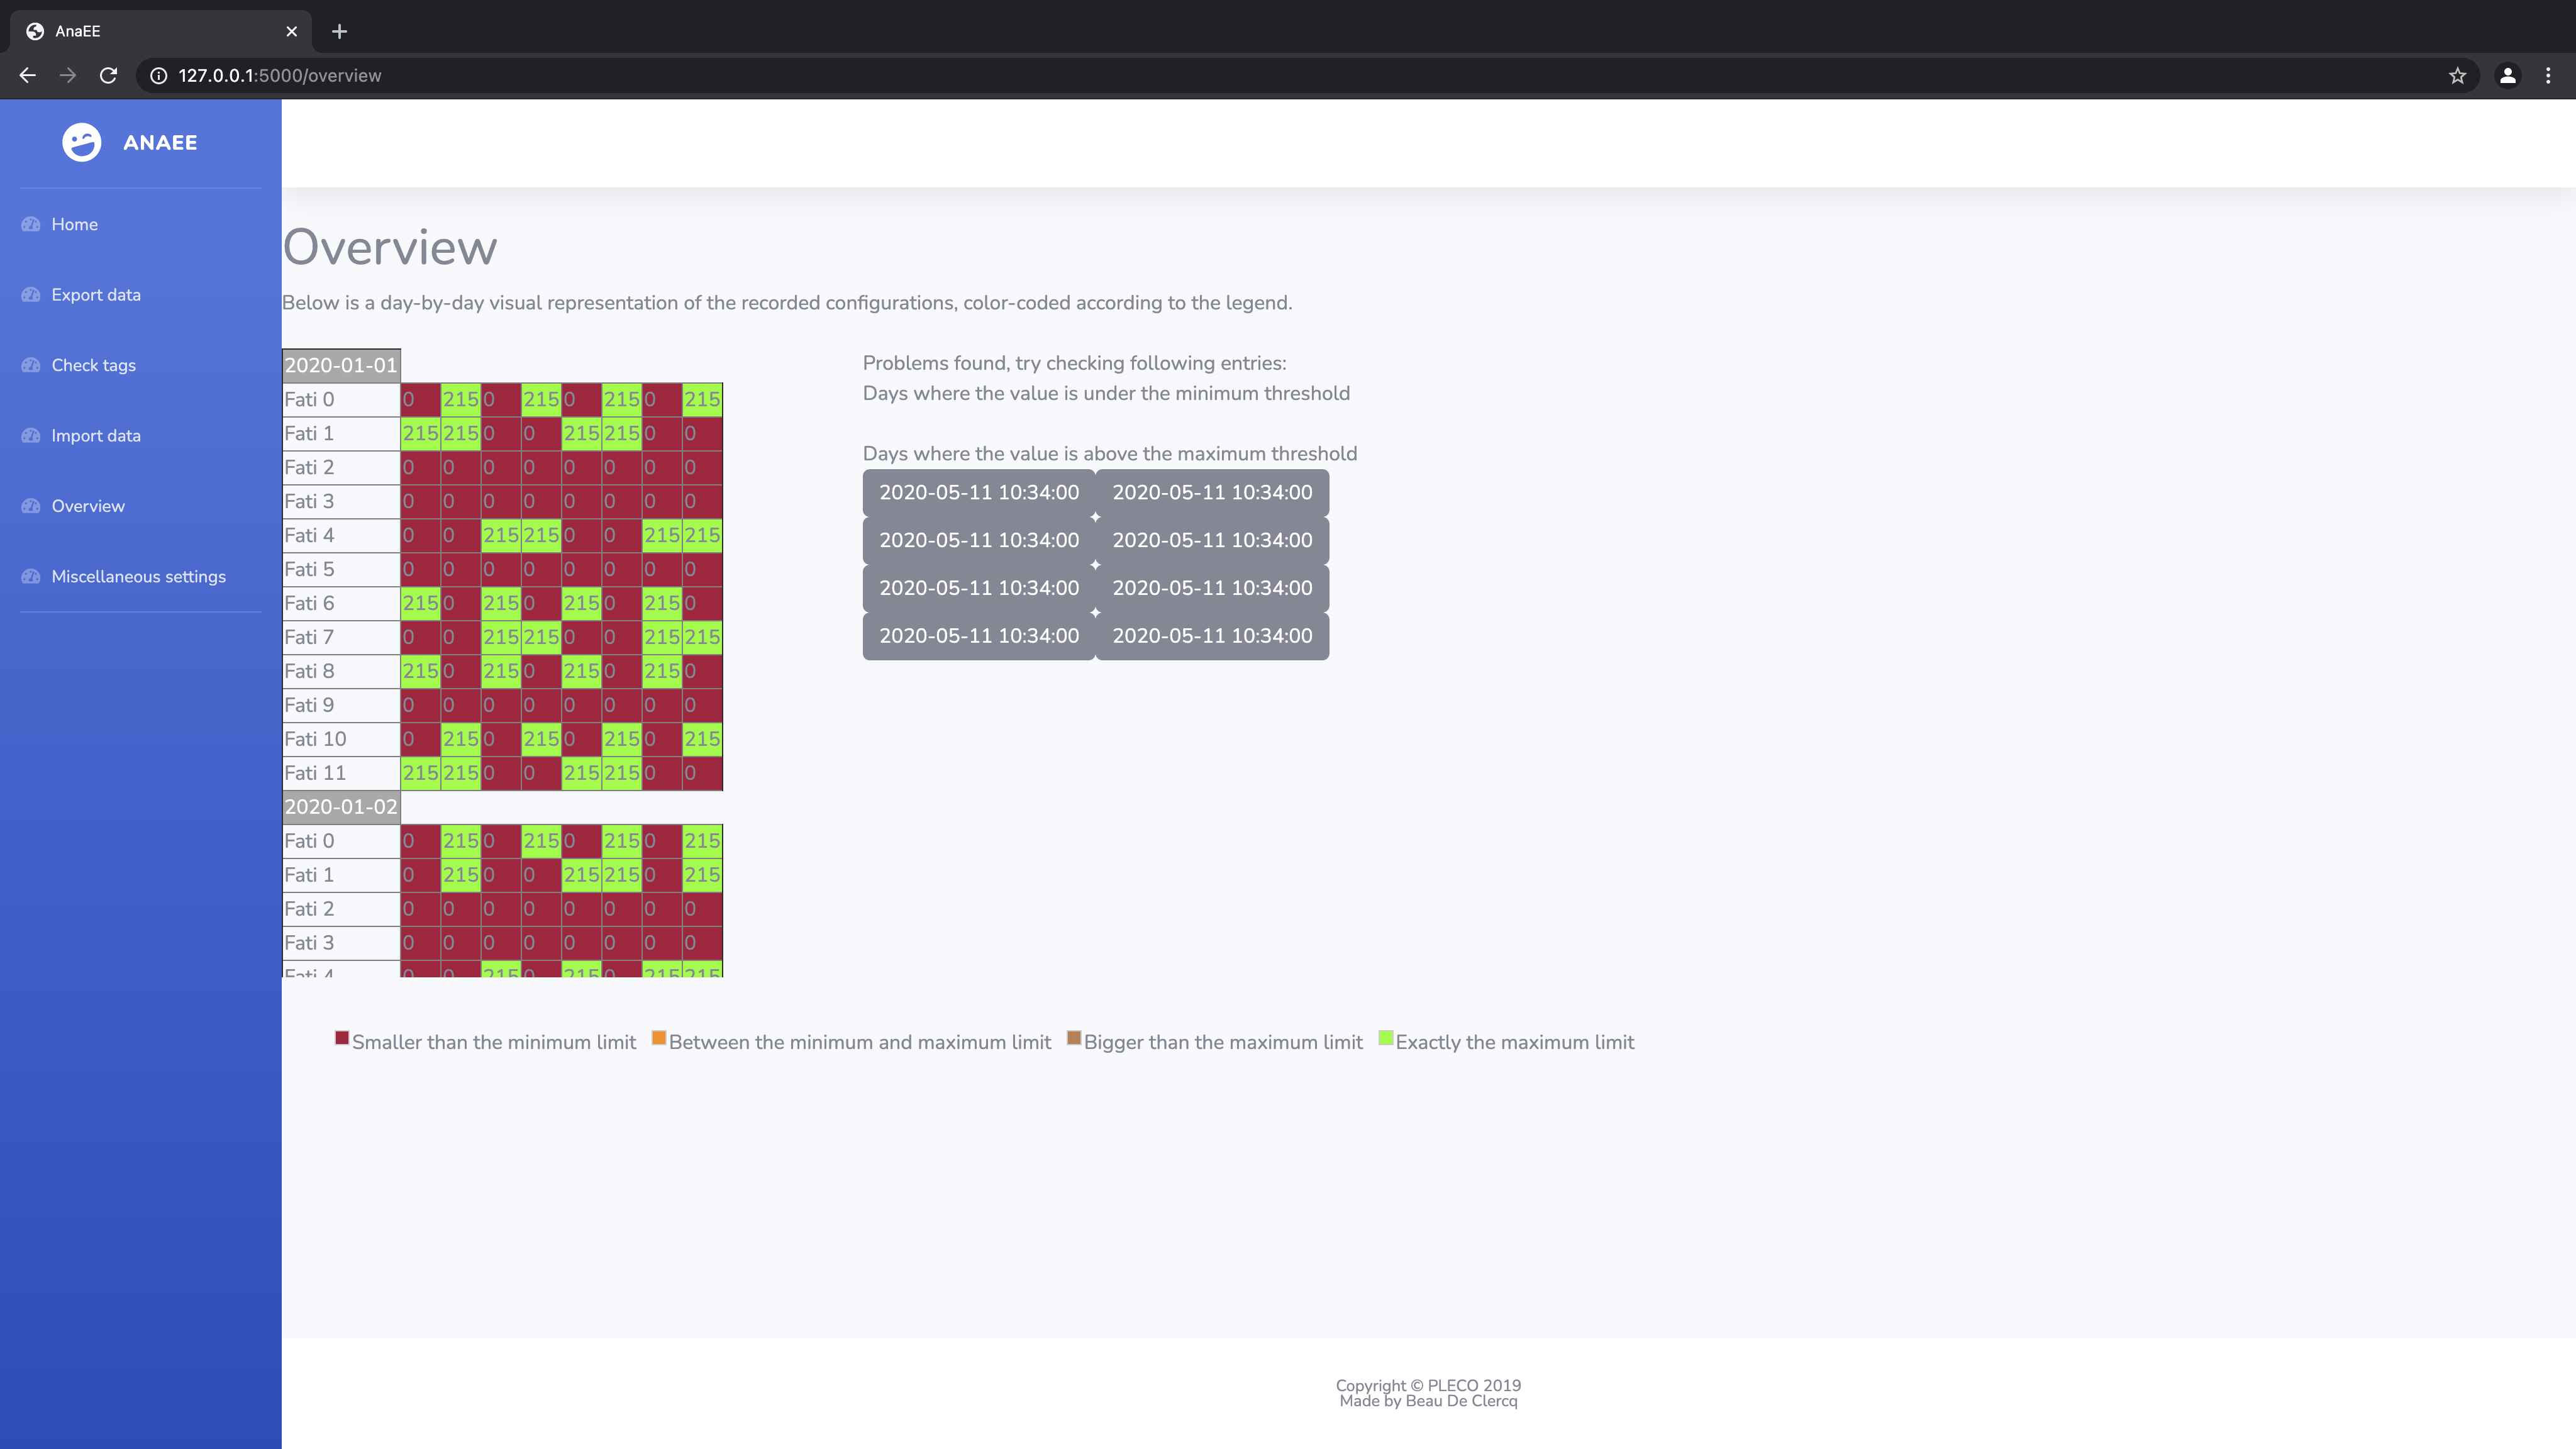
\includegraphics[width=\linewidth]{images/Overview.png}
	\captionof{figure}{Visual overview of the records}
\end{center}
In the \lq Overview\rq tab, the user can get a quick view at what the result is of all the records currently in the database.\\
In this overview, the user can see per day which valve is active for how long and whether it meets the required limits found in the \lq Miscellaneous\rq tab.\\

\subsection{Export the data}
\begin{center}
	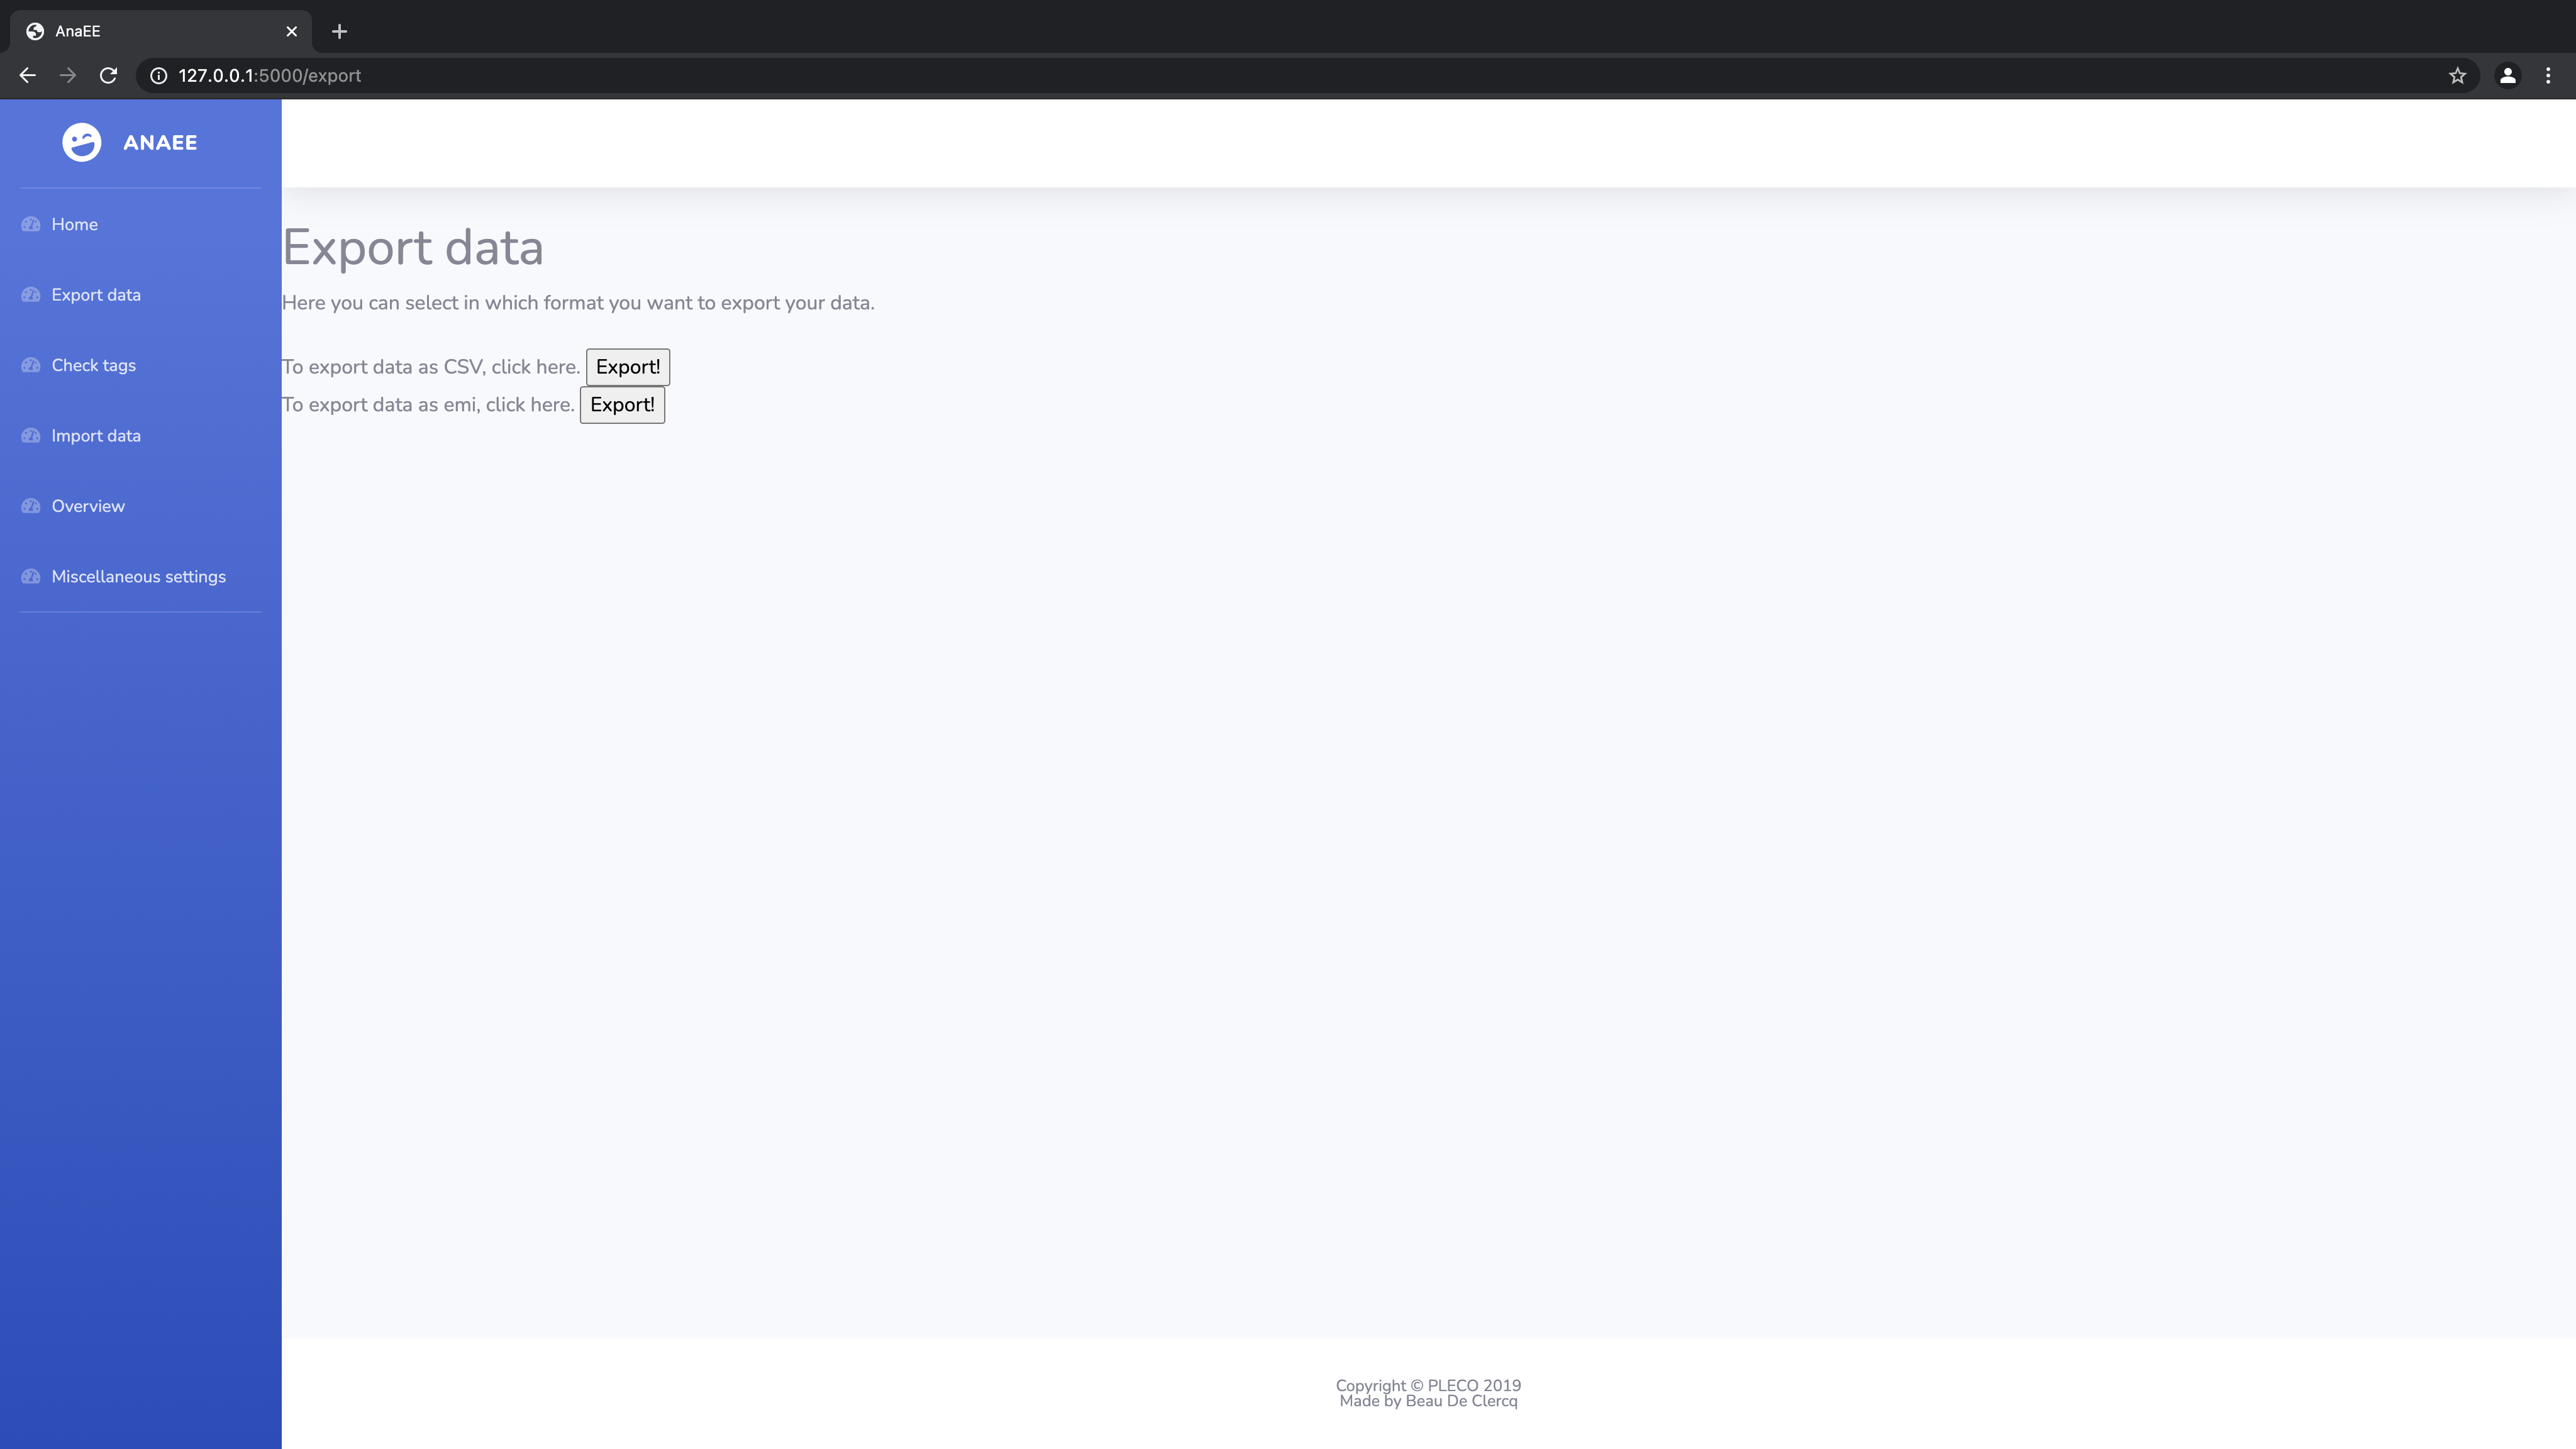
\includegraphics[width=\linewidth]{images/Export_data.png}
	\captionof{figure}{Data exportation}
\end{center}
In the \lq Export data\rq tab, the user can choose in which format he wants to export his data.\\
Selecting either option will open a file dialog where the user can select the file the data needs to be exported to.

\subsection{Import the data}
\begin{center}
	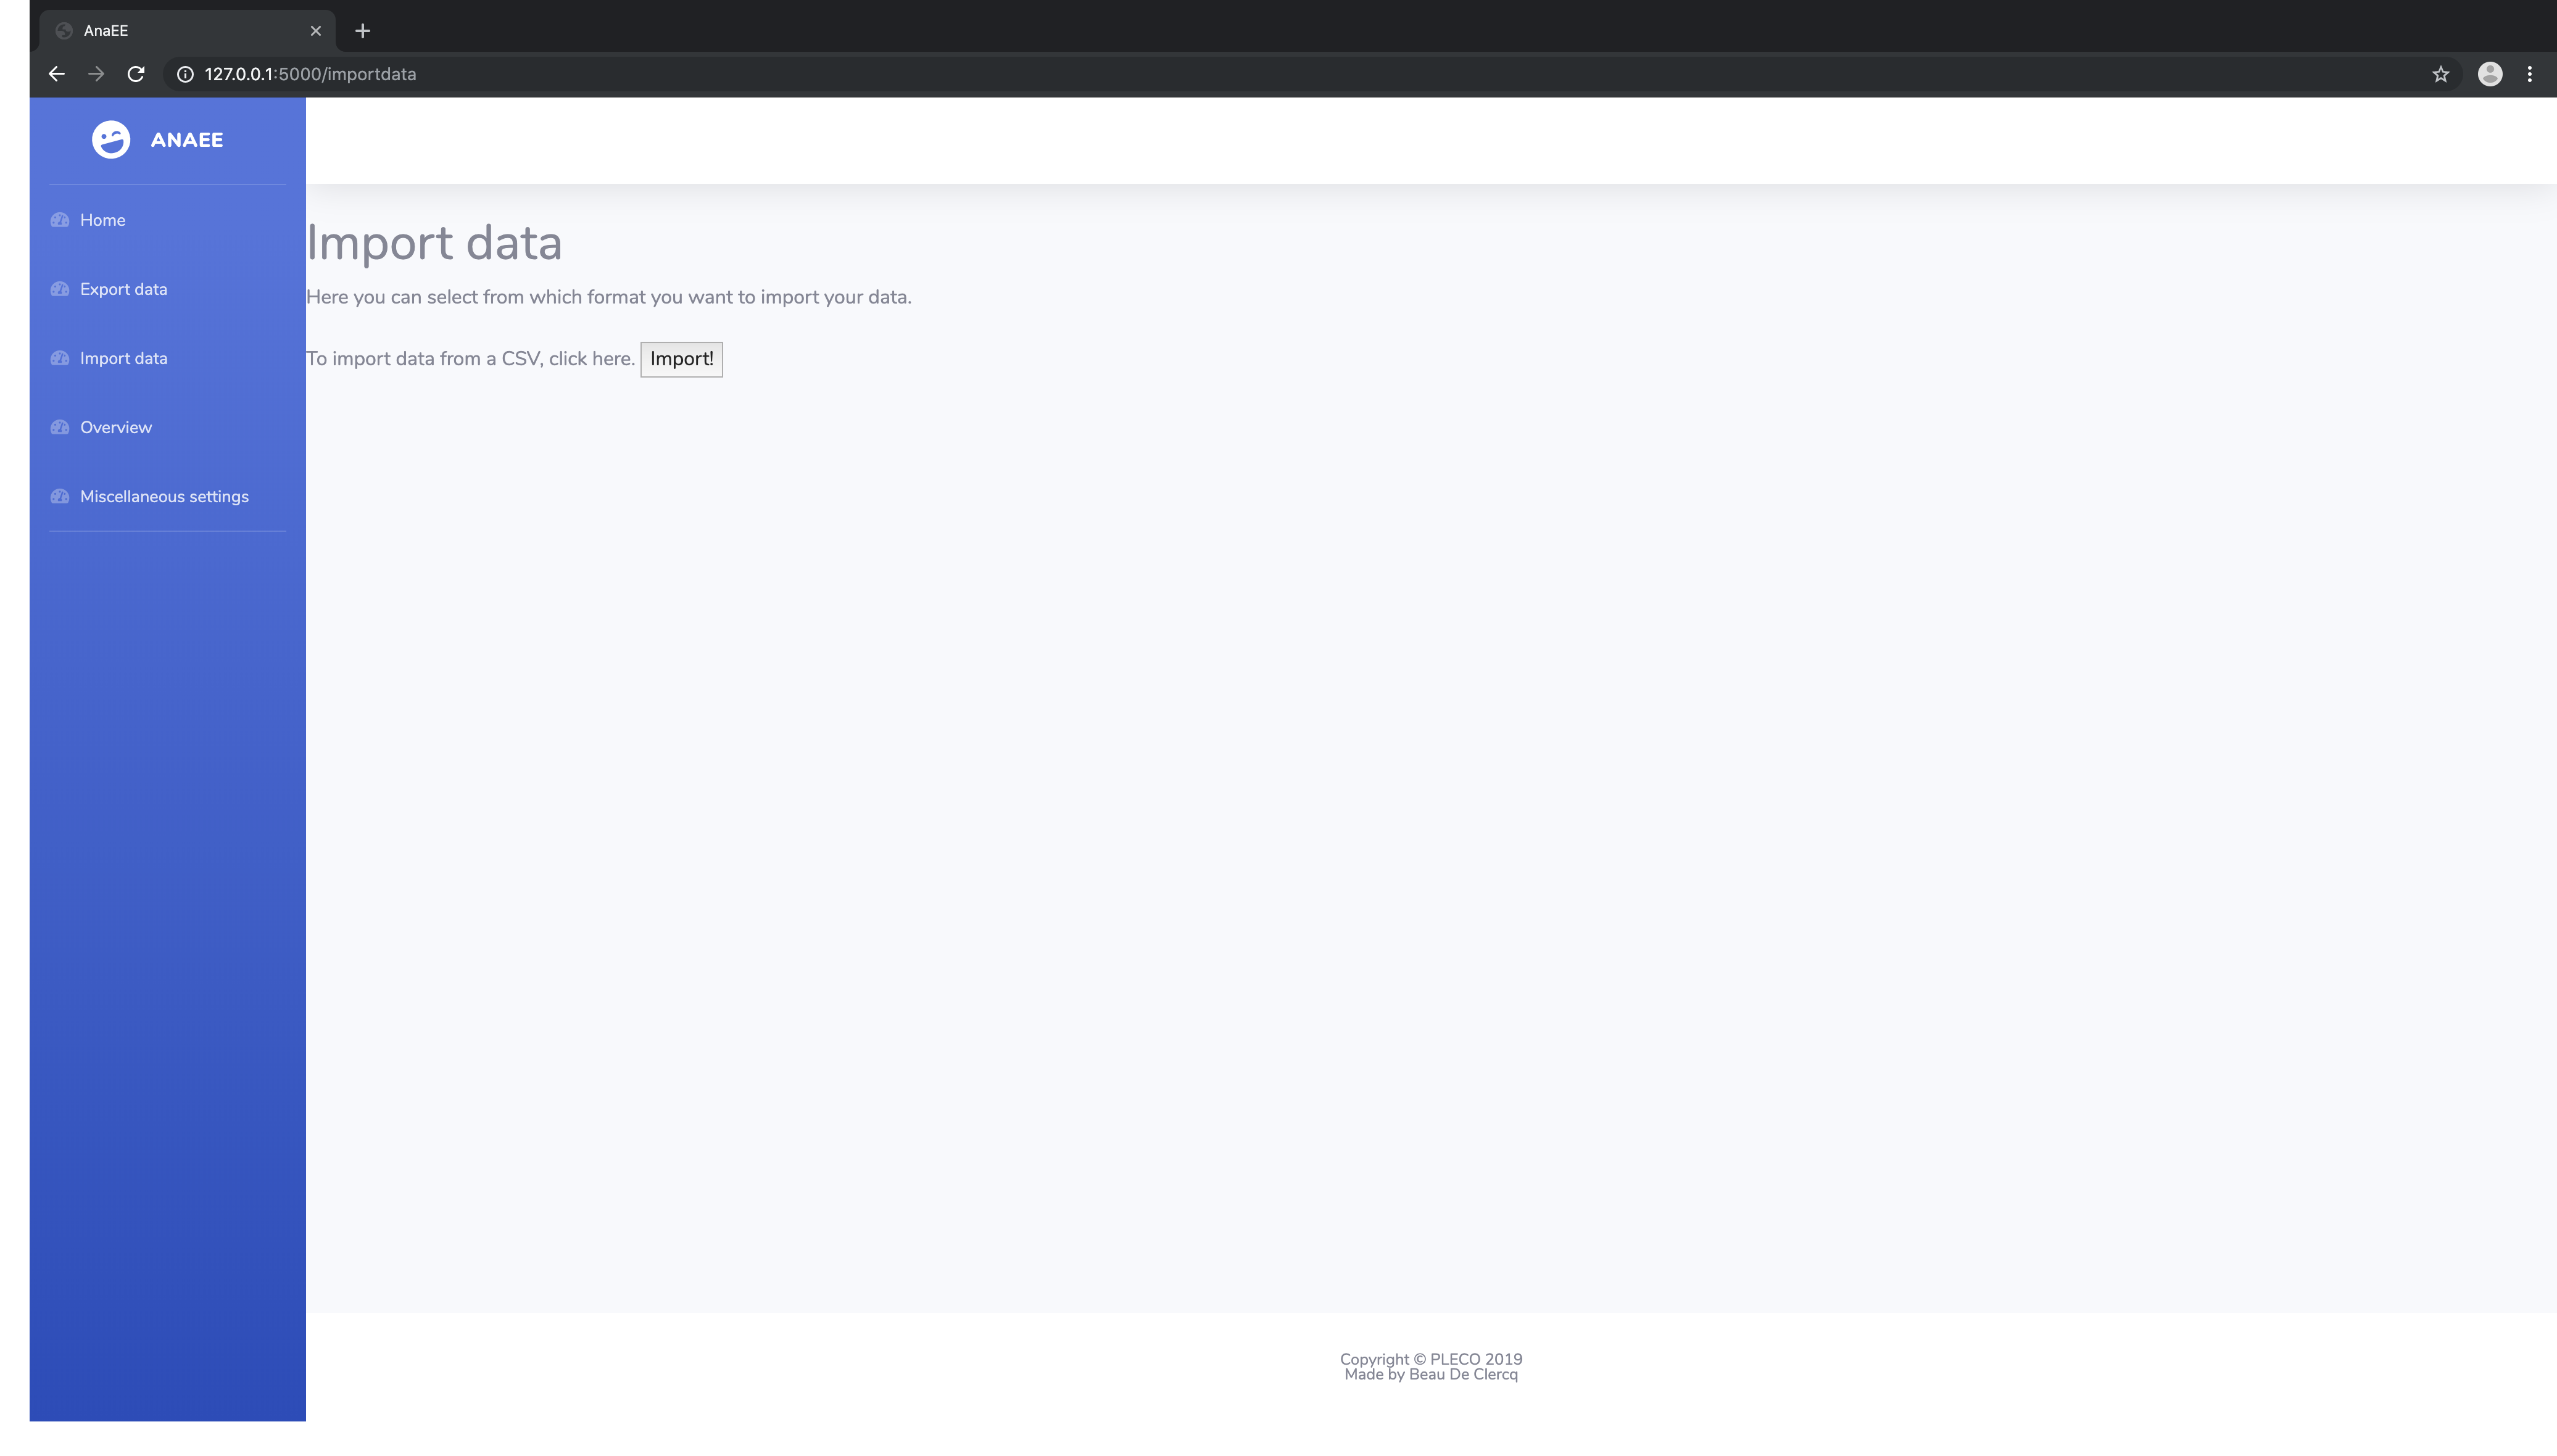
\includegraphics[width=\linewidth]{images/Import_data.png}
	\captionof{figure}{Data importing}
\end{center}
In the \lq Import data\rq tab, the user can choose from which format he wants to import his data.\\
Selecting either option will open a file dialog where the user can select the file the data needs to be imported from.

\subsection{Miscellaneous settings}
\begin{center}
	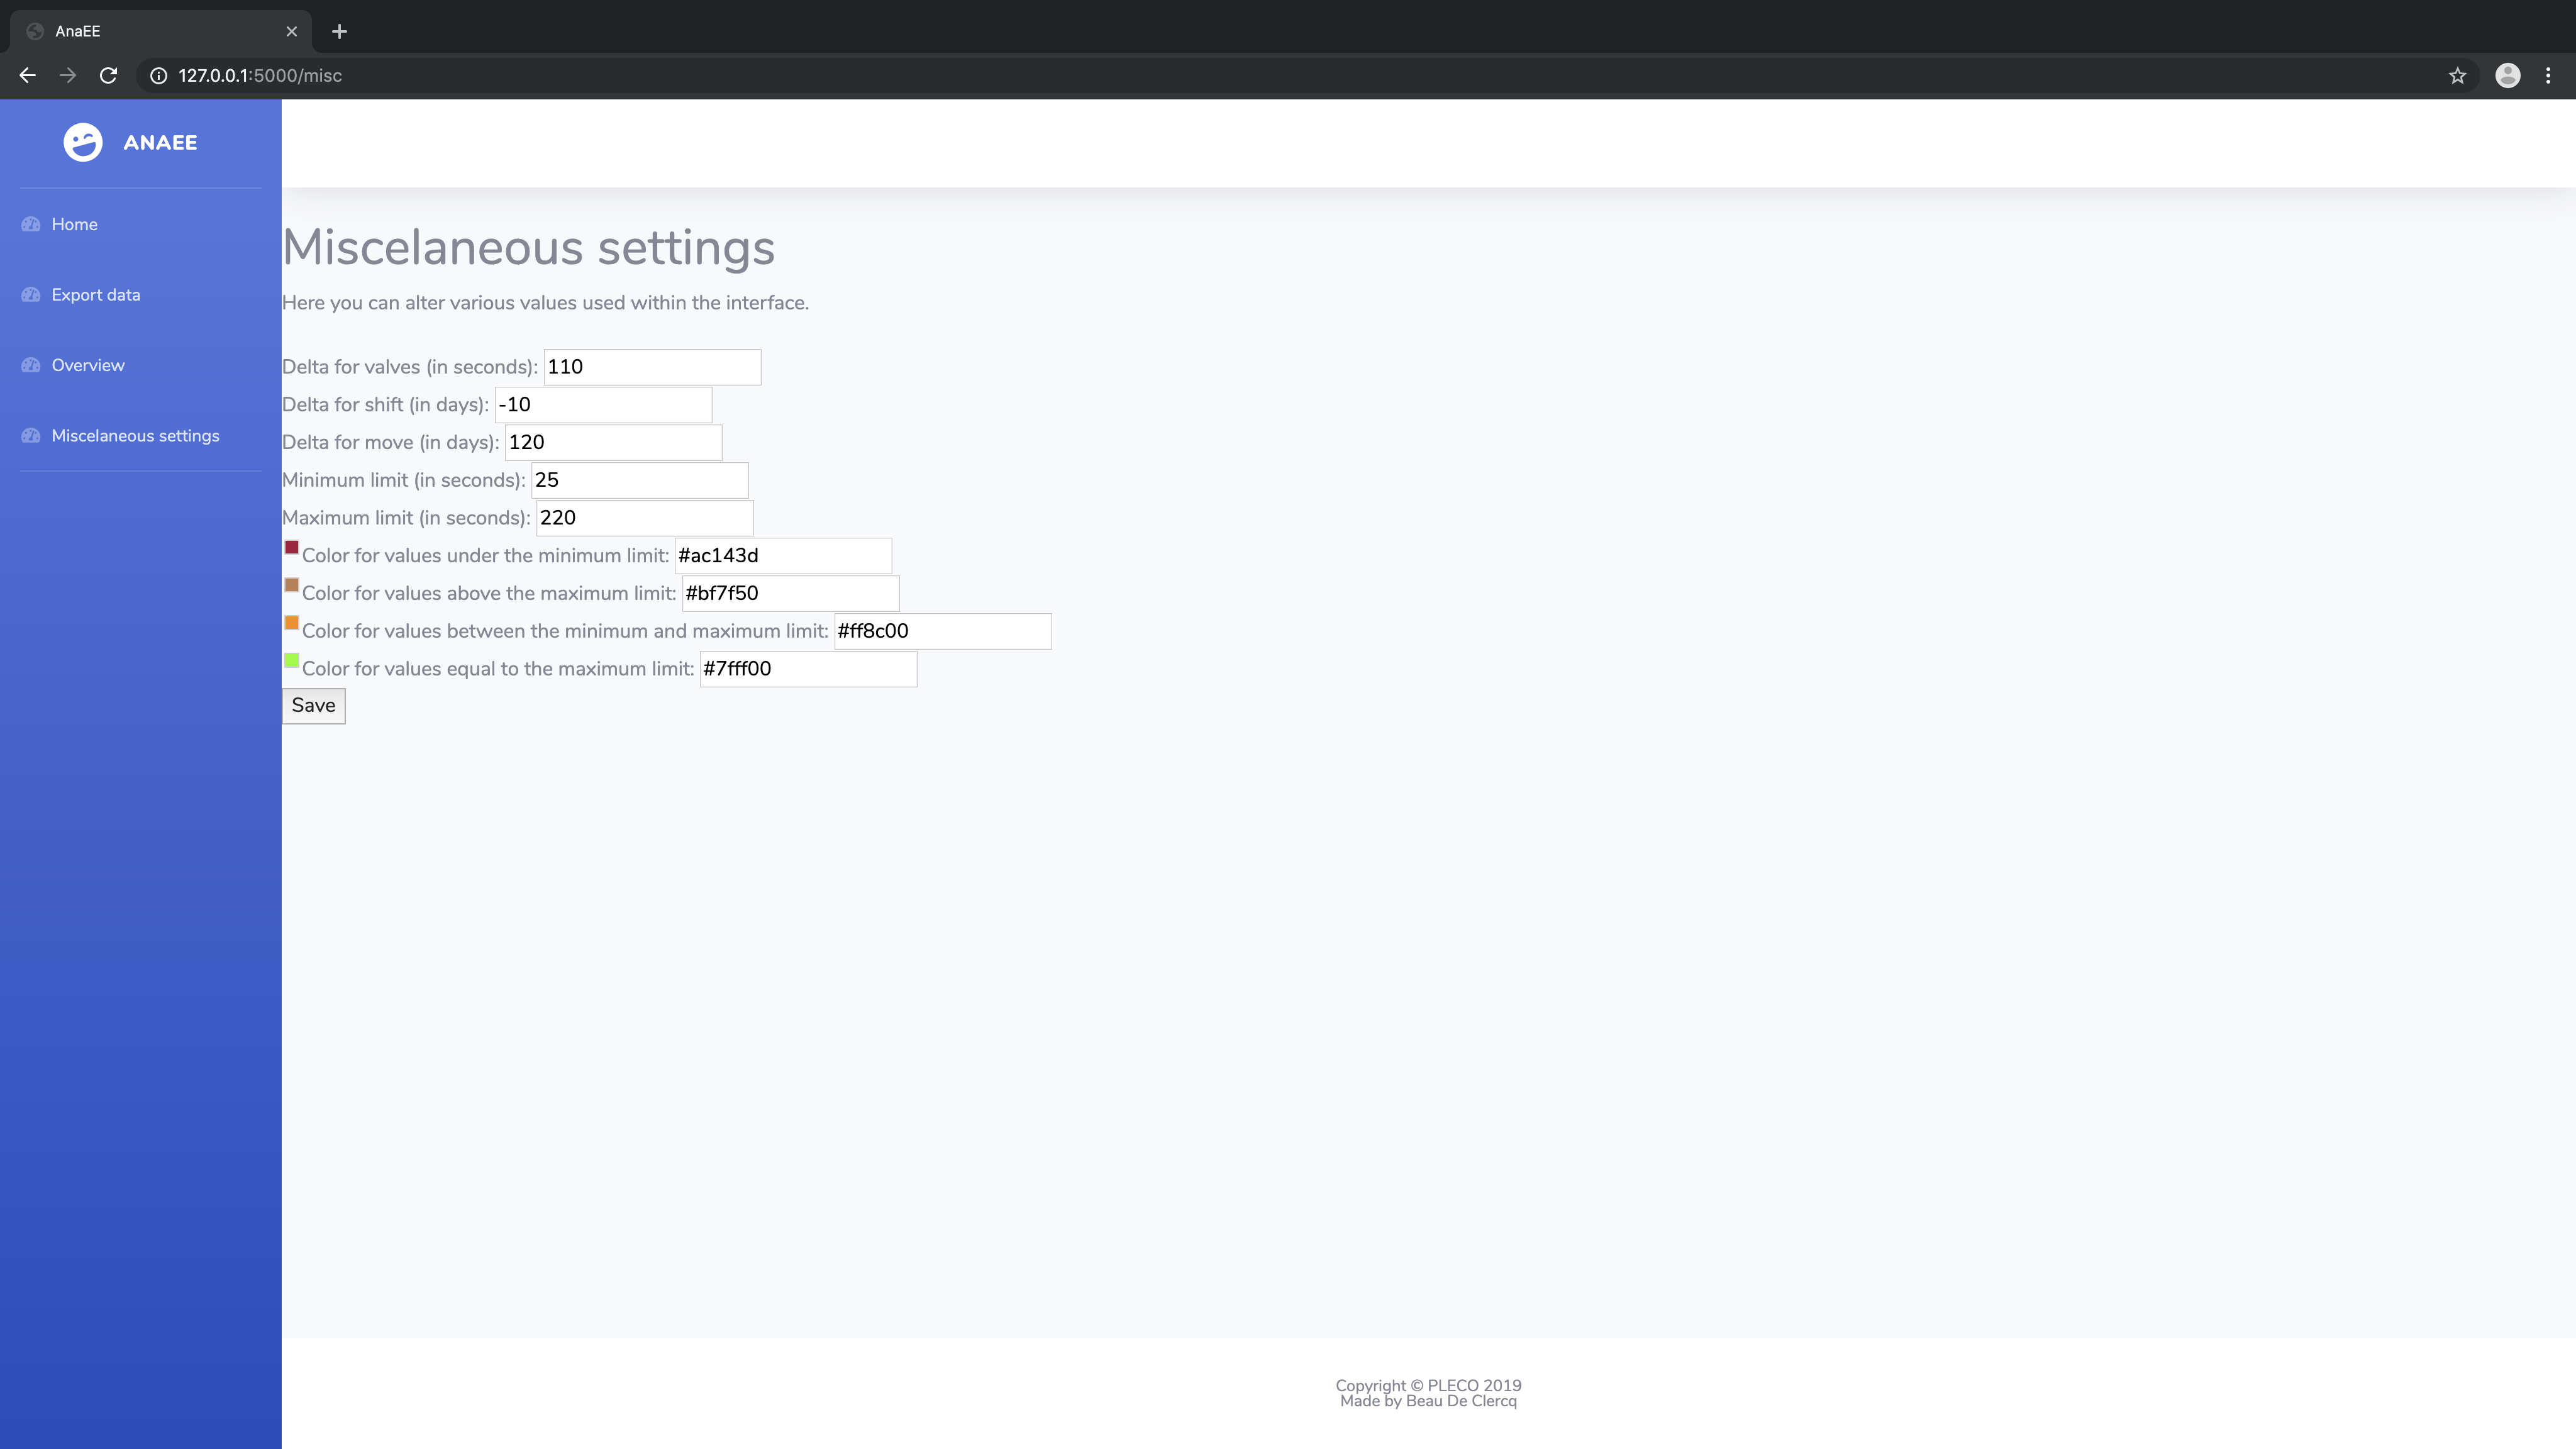
\includegraphics[width=\linewidth]{images/Misc_settings.png}
	\captionof{figure}{Miscelaneous settings for the interface}
\end{center}
In the tab \lq Miscellaneous settings\rq, a number of values can be adapted.
\begin{itemize}
	\item Delta for valves: this value specifies the amount of time that needs to be used when auto-generating an end-timestamp.
	\item Delta for shift: the amount of days used to shift a series of entries on the homepage.
	\item Delta for move: the amount of days used to duplicate a series of entries on the homepage.
	\item Minimum limit: the amount of time a valve needs to be minimally active on any given day.
	\item Maximum limit: the amount of time a valve can be maximally active on any given day.
	\item Colors: the colors used in the \lq Overview\rq tab.
\end{itemize}
%\maketitle{Setup}

\end{document}
